\chapter{Random Variables}

The exploration of random variables arises from the observation that, in various situations, we may not be concerned with the specific basic outcome of a random experiment. Instead, we are often interested in some numerical function derived from that outcome.  For instance, consider an experiment where a coin is tossed ten times. Rather than focusing on the exact sequence of heads and tails that appears—such as heads, tails, heads, heads, tails, etc.—the experimenter might be primarily interested in the total count of heads obtained.\\

This shift in focus allows us to encapsulate the randomness of the experiment in a more manageable and meaningful way, as we transform the complexity of individual outcomes into a single number that conveys essential information about the experiment's result.

\section{Introduction to Random Variables}

The term \textbf{random variable} can be misleading because it suggests that the variable itself is random, or that it varies in a typical sense. In fact, a random variable \( X \) is better understood as a function that maps elements from the sample space \( \Omega \) to the real numbers \( \mathbb{R} \). The term \textit{random} refers to the inherent uncertainty in selecting an element \( \omega \) from the sample space \( \Omega \). Once we fix an elementary outcome \( \omega \), the random variable assigns a specific real value, denoted \( X(\omega) \).\\

It is crucial to distinguish between the probability measure, which applies to subsets of the sample space (known as events), and the random variable, which is tied to each individual outcome \( \omega \). Not all subsets of the sample space qualify as events, and similarly, not every function from \( \Omega \) to \( \mathbb{R} \) is classified as a random variable. In particular, a random variable is defined as an \textbf{$\mathcal{F}$-measurable function}, as elaborated below.

\begin{definition}
    Consider a measurable space \( (\Omega, \mathcal{F}) \). A function \( f: \Omega \to \mathbb{R} \) is termed an \textbf{$\mathcal{F}$-measurable function} if the pre-image of every Borel set is an \textbf{$\mathcal{F}$-measurable} subset of \( \Omega \).
\end{definition}

To clarify, the pre-image of a Borel set \( B \) under the function \( f \) is defined as:

\[
f^{-1}(B) = \{ \omega \in \Omega \mid f(\omega) \in B \} 
\]


\begin{center}
    \begin{tikzpicture}[
        scale=1.2,
        >=stealth,
        event/.style={draw, minimum width=1.5cm, minimum height=1cm, fill=blue!10},
        borelset/.style={draw, minimum width=1.5cm, minimum height=1cm, fill=red!10},
        point/.style={circle, fill, inner sep=1pt},
        ]
    
        % Sample Space (Omega)
        \draw [rounded corners] (0,0) rectangle (5,5);
        \node[anchor=north west] at (0,5) {Sample Space $\Omega$};
    
        % F-measurable subset
        \draw [blue!40, pattern=north west lines, pattern color=blue!40] 
            (0.25,0.25) to[out=60,in=-120] (2,2) to[out=60,in=180] (3.5,3.5) 
            to[out=0,in=45] (3.5,1) to[out=225,in=0] (0.25,0.25);
        \node at (3,2) {$f^{-1}(B) \in \mathcal{F}$};
    
        % Points in Omega
        \node[point] (w1) at (1.5,1) {};
        \node[below left=2pt] at (w1) {$\omega_1$};
        \node[point] (w2) at (3,3) {};
        \node[above right=2pt] at (w2) {$\omega_2$};
    
        % Borel Set
        \draw[red!40, fill=red!10] (5.7,1) rectangle (6.3,3) 
            node[midway, right=0.3cm] {$B \in \mathcal{B}(\mathbb{R})$};
    
        % Real Line (R)
        \draw[->] (6,-0.5) -- (6,4.5) node[above] {$\mathbb{R}$};

        % Function mapping
        \draw[->, thick] (4,2) -- (5.7,2) node[midway, above] {$f$};

        % Additional Labels
        \node[text width=6cm] at (2.5,-0.5) 
            {$f$ is $\mathcal{F}$-measurable if $f^{-1}(B) \in \mathcal{F}$ for all $B \in \mathcal{B}(\mathbb{R})$};
    
        % Show function mapping for specific points
        \draw[->, dashed] (w1) to[out=0,in=180] (6,1);
        \draw[->, dashed] (w2) to[out=0,in=180] (6,3);
    \end{tikzpicture}
    \end{center}
    


\begin{definition}
    Consider a probability space \((\Omega, \mathcal{F}, P)\), where \(\Omega\) represents the sample space, \(\mathcal{F}\) is a \(\sigma\)-algebra of events, and \(P\) is a probability measure. A random variable \(X\) is defined as a function that maps elements from \(\Omega\) to the real numbers \(\mathbb{R}\), such that \(X\) is measurable with respect to \(\mathcal{F}\).
\end{definition}

To elaborate, this means that for any Borel set \(B\) (which belongs to the collection of Borel sets \(\mathcal{B}(\mathbb{R})\)), the pre-image of \(B\) under the random variable \(X\) must be an event in the \(\sigma\)-algebra \(\mathcal{F}\). In a visual sense, you can think of \(X\) as a mapping that takes each outcome \(\omega\) from the sample space \(\Omega\) and assigns it a value in the real line \(\mathbb{R}\).\\

Now, the set defined as \(\{ \omega \in \Omega \mid X(\omega) \in B \}\) represents an event in \(\mathcal{F}\) for every Borel set \(B\). This set corresponds to the outcomes for which the random variable \(X\) falls within the Borel set \(B\). As a result, since each such event has a probability associated with it, we can define what is known as the probability law of the random variable \(X\). This law encapsulates how probabilities are distributed across the possible values that \(X\) can take.\\

\begin{definition}
The \textbf{probability law}, denoted as \( P_X \), is defined as a function that maps Borel sets to probabilities, specifically:

\[
P_X : \mathcal{B}(\mathbb{R}) \to [0, 1]
\]

This means that for any Borel set \( B \) in \( \mathbb{R} \), the probability law is given by:

\[
P_X(B) = P(\{ \omega \in \Omega \mid X(\omega) \in B \})
\]

Here, \( P \) is the probability measure applied to the set of outcomes \( \omega \) in the sample space \( \Omega \) for which the random variable \( X \) falls within the set \( B \). 
\end{definition}

To clarify further, we can think of \( P_X \) as a composition of two functions: the probability measure \( P \) and the inverse image of \( X \), denoted as \( X^{-1} \). Mathematically, we express this relationship as:

\[
P_X(\cdot) = P \circ X^{-1}(\cdot)
\]

\vspace{10pt}
Notice that we are not saying $X^{-1}$ is an inverse function i.e., the random variable function $X$ is invertible. This is not the case. That's just the notation for the set of elements of the sample space that map to the Borel set $B$. So, $X^{-1}$ is the pre-image of $B$. Since $X$ is an $\mathcal{F}$-measurable function, $X^{-1}$ is the element of the $\text{Borel }\sigma$-algebra of $\Omega$.\\  

This relationship reveals that the probability law completely determines the statistical properties of the random variable \( X \). In other words, it tells us the likelihood of \( X \) taking values in any given Borel set \( B \).\\

To visualize this, consider that \( P \) represents the mapping from an event \( E \) to its associated probability. In contrast, \( P_X \) maps a Borel set \( B \) to the probability space, effectively combining the function \( P \) with the inverse image \( X^{-1} \). This process illustrates how the behavior of the random variable is encapsulated by its probability law.

\begin{center}
    \begin{tikzpicture}[
        scale=1.2,
        >=stealth,
        event/.style={draw, minimum width=1.5cm, minimum height=1cm, fill=blue!10},
        borelset/.style={draw, minimum width=1.5cm, minimum height=1cm, fill=red!10},
        point/.style={circle, fill, inner sep=1pt},
    ]
        % Define coordinates for the three main spaces
        \coordinate (prob_center) at (0,0);
        \coordinate (omega_center) at (6,0);
        \coordinate (real_center) at (12,0);
        
        % Probability interval [0,1] (left)
        \draw[->] (0,-2.4) -- (0,3) node[above] {$[0,1]$};
        \node at (0,-2.8) {Probability};
        
        % Sample Space (middle)
        \draw [rounded corners] (2.5,-2.5) rectangle (8.5,3.0);
        \node[anchor=north] at (5.5,3) {Sample Space $\Omega$};
        
        % Event in F (preimage)
        \draw [blue!40, pattern=north west lines, pattern color=blue!40] 
            (3.5,-1.75) to[out=60,in=-120] (6,0) to[out=60,in=180] (7.5,1.5) 
            to[out=0,in=45] (7.5,-1) to[out=225,in=0] (3.5,-1.75);
        \node at (5,0.5) {$X^{-1}(B) \in \mathcal{F}$};
        
        % Points in Omega
        \node[point] (w1) at (5.5,-1) {};
        \node[below left=2pt] at (w1) {$\omega_1$};
        \node[point] (w2) at (7,1) {};
        \node[above right=2pt] at (w2) {$\omega_2$};
        
        % Borel Set
        \draw[red!40, fill=red!10] (11.0,-1) rectangle (12,1) 
            node[midway, right=0.5cm] {$B$};

        % Real Line (right)
        \draw[->] (11.5,-3) -- (11.5,3) node[above] {$\mathbb{R}$};
        \node[anchor=south] at (10.6,-2.8) {$(\mathbb{R}, \mathcal{B}(\mathbb{R}))$};
        
        % Random Variable mapping (Omega to R)
        \draw[->, thick] (8.5,0) -- (11,0) node[midway, above] {$X$};
        
        % Probability measure mapping (X^-1(B) to [0,1])
        \draw[->, thick, blue] (4.25,-1) -- (0,-1) node[midway, above] {$P_X = P \circ X^{-1}$};
        
        % Show function mapping for specific points
        \draw[->, dashed] (w1) to[out=0,in=180] (12,-1);
        \draw[->, dashed] (w2) to[out=0,in=180] (12,1);
        
        % Additional Labels
        \node[text width=14cm] at (7.5,-3) 
            {$P_X(B) = (P \circ X^{-1})(B) = P(\{\omega \in \Omega : X(\omega) \in B\})$};
    
    \end{tikzpicture}
\end{center}

\begin{theorem}
    Let \((\Omega, \mathcal{F}, P)\) be a probability space, and let \(X\) be a real-valued random variable. Then, the probability law \(P_X\) of \(X\) is a probability measure on \((\mathbb{R}, \mathcal{B}(\mathbb{R}))\).
\end{theorem}

\begin{proof}
We need to show that \(P_X\) is indeed a probability measure on \((\mathbb{R}, \mathcal{B}(\mathbb{R}))\). \\

1. \textbf{Non-negativity:} For any Borel set \(B\), since \(P\) is a probability measure, we have:
   \[
   P_X(B) = P(X^{-1}(B)) \geq 0.
   \]

2. \textbf{Normalization:} The total measure of the whole space must equal 1. Since \(X\) can take any value in \(\mathbb{R}\), we have:
   \[
   P_X(\mathbb{R}) = P(X^{-1}(\mathbb{R})) = P(\Omega) = 1.
   \]

3. \textbf{Countable Additivity:} For any countable collection of disjoint Borel sets \(B_1, B_2, \ldots\) (i.e., \(B_i \cap B_j = \emptyset\) for \(i \neq j\)), we have:
   \[
   P_X\left(\bigcup_{i=1}^\infty B_i\right) = P(X^{-1}(\bigcup_{i=1}^\infty B_i)) = P\left(\bigcup_{i=1}^\infty \{ \omega \in \Omega : X(\omega) \in B_i \}\right).
   \]
   By the countable additivity of \(P\), this can be rewritten as:
   \[
   P\left(\bigcup_{i=1}^\infty \{ \omega \in \Omega : X(\omega) \in B_i \}\right) = \sum_{i=1}^\infty P\left(\{ \omega \in \Omega : X(\omega) \in B_i \}\right) = \sum_{i=1}^\infty P_X(B_i).
   \]

Since all three properties of a probability measure hold, we conclude that \(P_X\) is indeed a probability measure on \((\mathbb{R}, \mathcal{B}(\mathbb{R}))\). 
\end{proof}

\textbf{Note:} If $\Omega$ is countable set, then $\mathcal{F}$ can be taken as $2^\Omega$. Typical example is the \textit{discrete probability space}. In that case, all functions from $\Omega$ to $\mathbb{R}$ will be random variables because you cannot have a pre-image which is not $\mathcal{F}$-measurable, So, only in cases where $\mathcal{F}$ is not $2^\Omega$ is there a possibility that a function is not a random variable.\\

What we are interested now is - \textit{what values $X$ can take?} To be able to describe that, we will need to specify $P_X$ for all Borel sets. Then, we will know the complete probabilistic description of the random variable on the real line. It turns out, you don't need $P_X$ for all Borel sets. It is enough to specify $P_X$ for certain \textit{nice} sets. Let's see how we do that.\\

Recall when we were generating the Borel $\sigma$-algebra on the real line, we mentioned that there are multiple ways of generating it. One of them is using \textit{open intervals}. The other important way is to use \textit{semi-infinite intervals}. We can look at the $\mathcal{B}(\mathbb{R})$ as being generated by the sets of form $(-\infty, x] \text{ where x } \in \mathbb{R}$.\\

What are we trying to get at is - \textit{the probability law that is defined for all Borel sets must also be defined for the generating class}. Thus, $P_X((-\infty, x])$ is well-defined for all $x \in \mathbb{R}$. Another way of writing  $P_X((-\infty, x])$ is  $P_X({\omega \in \Omega | X(\omega) \leq x})$. This probability has a special name called \textbf{cumulative distribution function (CDF)}, often denoted by $F_X(x)$.\\

So, if you provide the probability law for all Borel sets, we can easily figure out the CDF. What is not so obvious and requires a proof is \textit{if you specify the CDF, you can specify the probability law for all Borel sets.} From the \textit{Classical Probability}, we know that if we get the CDF of a random variable, we know everything about it. This is a correct concept but not so obvious. Because to know everything about the random variable, we must know probability measure of all the Borel sets. The reason this is possible is because all the other Borel sets you can write as the countable intersections and unions of the generating class, and we can figure out $P_X$ from $F_X$. The way to formalize this notion is by using an object called \textit{$\pi$-system.}\\

\begin{definition}
    Given a set \(\Omega\), a \(\pi\)-system on \(\Omega\) is a non-empty collection of subsets of \(\Omega\) that remains stable under finite intersections. \\
    
    Formally, if we denote this collection by \(\mathcal{P}\), then \(\mathcal{P}\) is a \(\pi\)-system if, for any subsets \(A\) and \(B\) in \(\mathcal{P}\), the intersection \(A \cap B\) also belongs to \(\mathcal{P}\). This stability under intersection is a key property that defines \(\pi\)-systems.
\end{definition}

Just like $\sigma$-algebra, $\pi$-system is another algebraic structure. $\pi$-systems require closure under only finite intersections - no complements or no countable unions. So, this structure is much weaker than $\sigma$-algebra. In fact, it is also much weaker than the \textit{algebra}. All algebras are clearly $\pi$-systems, but not the other way around.\\

A particularly common example of a \(\pi\)-system on \(\mathbb{R}\) (the set of real numbers) is the collection of all closed semi-infinite intervals of the form \((-\infty, x]\) where \(x\) is any real number. We denote this class as \(\pi(\mathbb{R})\), and express it mathematically by:
\[
\pi(\mathbb{R}) = \{ (-\infty, x] : x \in \mathbb{R} \}.
\]
This \(\pi\)-system is useful because each interval in \(\pi(\mathbb{R})\) represents a closed set extending infinitely to the left and bounded by a specific real number \(x\) on the right. The intervals in \(\pi(\mathbb{R})\) share the \(\pi\)-system property: if we take any two intervals \((-\infty, x_1]\) and \((-\infty, x_2]\) from \(\pi(\mathbb{R})\), their intersection will also be of the same form, specifically \((-\infty, \min(x_1, x_2)]\), which again belongs to \(\pi(\mathbb{R})\).\\

\begin{lemma}
    The \textbf{Borel} $\sigma$-\textbf{algebra} on a set $R$, often denoted by $\mathcal{B}(R)$, is the smallest $\sigma$-algebra containing all sets in a collection $\pi(R)$. We write this relation as:
\[
\mathcal{B}(R) = \sigma(\pi(R)),
\]
where $\sigma(\pi(R))$ represents the $\sigma$-algebra generated by $\pi(R)$. Here, $\pi(R)$ is called a $\pi$-\textbf{system} on $R$, which is simply a collection of subsets of $R$ closed under finite intersections. 
\end{lemma}

To deepen our understanding, let us consider an important result from \textbf{measure theory} regarding such $\pi$-systems. Suppose we have two \textbf{finite measures}, say $\mu$ and $\nu$, defined on a measurable space $(R, \sigma(\pi(R)))$. Now, if $\mu$ and $\nu$ \textbf{agree} on $\pi(R)$ (that is, $\mu(A) = \nu(A)$ for every $A \in \pi(R)$), then this result guarantees that $\mu$ and $\nu$ will also agree on the entire $\sigma$-algebra $\sigma(\pi(R))$. In other words, for every $B \in \sigma(\pi(R))$, it follows that:
\[
\mu(B) = \nu(B).
\]

This result is powerful because it tells us that to verify equality of two finite measures on the entire $\sigma$-algebra $\sigma(\pi(R))$, it suffices to verify their equality on the simpler structure of the $\pi$-system $\pi(R)$. This principle often simplifies work with measures by reducing the complexity of the verification needed, allowing us to focus on a smaller collection of sets.\\

\begin{lemma}
    Let $\Omega$ be a set and consider a $\pi$-system $\mathcal{P}$ over $\Omega$. Specifically, if $A, B \in \mathcal{P}$, then $A \cap B \in \mathcal{P}$ as well. We denote by $\Sigma = \sigma(\mathcal{P})$ the $\sigma$-algebra generated by $\mathcal{P}$. The $\sigma$-algebra $\Sigma$ includes all subsets of $\Omega$ that can be formed by countable unions, intersections, and complements of elements in $\mathcal{P}$.
\end{lemma}

\begin{proof}
Let $\mu_1$ and $\mu_2$ be two measures defined on the measurable space $(\Omega, \Sigma)$ that agree on a few conditions:\\

1. Both measures are finite on $\Omega$, meaning $\mu_1(\Omega) = \mu_2(\Omega) < \infty$.\\
2. The measures agree on $\mathcal{P}$, so $\mu_1(A) = \mu_2(A)$ for all $A \in \mathcal{P}$.\\

Our goal is to show that these conditions imply $\mu_1 = \mu_2$ on all of $\Sigma$, not just on $\mathcal{P}$.\\

The key idea here leverages the fact that $\mathcal{P}$ is a $\pi$-system. Intuitively, because $\mathcal{P}$ is closed under intersections, it forms a structure that allows the agreement of $\mu_1$ and $\mu_2$ on $\mathcal{P}$ to extend naturally to all of $\Sigma$. This result is a powerful extension theorem for measures, which can be formally stated as follows:\\

If two measures $\mu_1$ and $\mu_2$ agree on a $\pi$-system $\mathcal{P}$ and are finite on $\Omega$, then they must agree on the entire $\sigma$-algebra $\Sigma = \sigma(\mathcal{P})$. That is,
\[
\mu_1(E) = \mu_2(E) \quad \text{for all } E \in \Sigma.
\]

\textit{Why does this work?} The reasoning involves verifying that the set of all $E \in \Sigma$ for which $\mu_1(E) = \mu_2(E)$ forms a $\lambda$-system (also called a Dynkin system). A $\lambda$-system is a collection of sets closed under complements and countable disjoint unions, and every $\pi$-system is also contained within a $\lambda$-system that forms a $\sigma$-algebra. Thus, the combination of the $\pi$-system and the $\lambda$-system properties leads to the conclusion that $\mu_1 = \mu_2$ on $\Sigma$.
\end{proof}

\begin{corollary}
    If two probability measures agree on a $\pi$-system, then they agree on the $\sigma$-algebra generated by that $\pi$-system.
\end{corollary}

We will use this result to prove the theorem on CDF.

\subsection{Cumulative Distribution Function}

Consider the \textit{Probability Space} \((\Omega, \mathcal{F}, P)\) and a random variable \(X : \Omega \to \mathbb{R}\). This mapping \(X\) induces a new probability space \((\mathbb{R}, \mathcal{B}(\mathbb{R}), P_X)\) on the real line, where \(\mathcal{B}(\mathbb{R}) = \sigma(\pi(\mathbb{R}))\) is the Borel \(\sigma\)-algebra generated by the collection of semi-infinite intervals on \(\mathbb{R}\), i.e., the family \(\{(-\infty, x] : x \in \mathbb{R}\}\).\\
  
For any \(x \in \mathbb{R}\), we know:
\[
(-\infty, x] \in \mathcal{B}(\mathbb{R}) \Rightarrow X^{-1}((-\infty, x]) \in \mathcal{F}.
\]
Thus, it is meaningful to consider the probability measure \(P_X\) applied to these intervals, and we define the \textbf{Cumulative Distribution Function (CDF)} of \(X\) as:
\[
F_X(x) = P_X((-\infty, x]) = P(\{\omega \in \Omega : X(\omega) \leq x\}), \quad x \in \mathbb{R}.
\]
For convenience, we denote \(P(X \leq x)\) as shorthand for \(P(\{\omega \in \Omega : X(\omega) \leq x\})\), though this is slightly informal notation.

\begin{theorem}
    The probability law \(P_X\) of the random variable \(X\) is completely characterized by its CDF \(F_X\). In other words, if two random variables \(X\) and \(Y\) have the same CDF, then they have the same probability law.
\end{theorem}

\begin{proof}
    Let \(\mathcal{P} = \{(-\infty, x] : x \in \mathbb{R}\}\). This is a \(\pi\)-system on \(\mathbb{R}\) because the intersection of any two intervals in \(\mathcal{P}\) is again an interval in \(\mathcal{P}\), i.e., if \(x \leq y\), then:
   \[
   (-\infty, x] \cap (-\infty, y] = (-\infty, \min(x, y)] \in \mathcal{P}.
   \]

   The Borel \(\sigma\)-algebra \(\mathcal{B}(\mathbb{R})\) is generated by \(\mathcal{P}\), so \(\mathcal{B}(\mathbb{R}) = \sigma(\mathcal{P})\).\\

   By the properties of a \(\pi\)-system and the extension theorem, any two probability measures on \((\mathbb{R}, \mathcal{B}(\mathbb{R}))\) that agree on the generating \(\pi\)-system \(\mathcal{P}\) must agree on the entire \(\sigma\)-algebra \(\mathcal{B}(\mathbb{R})\).\\

   Since \(F_X(x) = P_X((-\infty, x])\) uniquely determines the probability on each interval \((-\infty, x] \in \mathcal{P}\), the probability law \(P_X\) is fully determined by \(F_X\). Therefore, the CDF \(F_X\) uniquely characterizes the probability distribution of the random variable \(X\), as claimed.
\end{proof}

\subsection{Properties of CDF}

Let \( X \) be a random variable with cumulative distribution function (CDF) \( F_X(\cdot) \). 

\begin{theorem}
    The CDF \( F_X(x) \) is \textbf{monotonically non-decreasing}. Specifically, if \( x \leq y \), then \( F_X(x) \leq F_X(y) \).    
\end{theorem}

\begin{proof}
    The CDF at a point \( x \), \( F_X(x) \), is the probability that the random variable \( X \) takes a value less than or equal to \( x \). In other words,
\[
F_X(x) = P(X \leq x).
\]

Now, if \( x \leq y \), we want to show that \( F_X(x) \leq F_X(y) \). 

This will follow from a property of sets and probability measures. Observe that the set of outcomes where \( X \leq x \) is always contained within the set where \( X \leq y \) whenever \( x \leq y \). Formally, we have
\[
\{\omega \mid X(\omega) \leq x\} \subseteq \{\omega \mid X(\omega) \leq y\}.
\]
This inclusion tells us that every outcome that satisfies \( X \leq x \) also satisfies \( X \leq y \) when \( x \leq y \).

Now, probability measures are \textbf{monotonic} with respect to sets: if one set is contained within another, then the probability of the smaller set is less than or equal to the probability of the larger set. Applying this to our situation, we get
\[
P(X \leq x) \leq P(X \leq y).
\]
Thus, we conclude that
\[
F_X(x) \leq F_X(y),
\]
proving that \( F_X \) is indeed a monotonically non-decreasing function.
\end{proof}

\begin{theorem}
    \[
\lim_{x \to \infty} F_X(x) = 1 \quad \text{and} \quad \lim_{x \to -\infty} F_X(x) = 0.
\]
\end{theorem}

\begin{proof}
To understand this result, let's carefully examine what happens to the cumulative distribution function (CDF) \( F_X(x) = P(X \leq x) \) as \( x \) approaches \( -\infty \) and \( +\infty \).\\

First, let's consider:
\[
\lim_{x \to -\infty} F_X(x).
\]

This limit represents the probability that \( X \) takes on a value less than or equal to a very large negative number, which we expect to approach zero. We can see why by breaking down the steps:\\

1. By definition of the CDF, we have:
   \[
   \lim_{x \to -\infty} F_X(x) = \lim_{x \to -\infty} P(X \leq x).
   \]

2. Now, let's take a sequence \( \{ x_n \}_{n \in \mathbb{N}} \) where each \( x_n \) is smaller than the last, and this sequence decreases to \( -\infty \). Thus:
   \[
   \lim_{n \to \infty} P(X \leq x_n).
   \]

3. Observe that \( P(X \leq x_n) \) corresponds to the event \(\bigcap_{n \in \mathbb{N}} \{ \omega : X(\omega) \leq x_n \} \), which becomes smaller and smaller as \( x_n \) goes to \( -\infty \), eventually approaching the empty set, \(\emptyset\). So, we get:
   \[
   P\left( \bigcap_{n \in \mathbb{N}} \{ \omega : X(\omega) \leq x_n \} \right) = P(\emptyset) = 0.
   \]

Thus:
\[
\lim_{x \to -\infty} F_X(x) = 0.
\]

Now, let's use similar reasoning to evaluate \( \lim_{x \to \infty} F_X(x) \):\\

1. Again by the CDF definition,
   \[
   \lim_{x \to \infty} F_X(x) = \lim_{x \to \infty} P(X \leq x).
   \]

2. Now consider a sequence \( \{ x_n \}_{n \in \mathbb{N}} \) where each \( x_n \) is greater than the last, and this sequence increases to \( +\infty \):
   \[
   \lim_{n \to \infty} P(X \leq x_n).
   \]

3. In this case, \( P(X \leq x_n) \) corresponds to the event \(\bigcup_{n \in \mathbb{N}} \{ \omega : X(\omega) \leq x_n \}\), which approaches the entire sample space \(\Omega\) as \( x_n \) becomes very large.

Thus:
\[
P\left( \bigcup_{n \in \mathbb{N}} \{ \omega : X(\omega) \leq x_n \} \right) = P(\Omega) = 1.
\]

Therefore:
\[
\lim_{x \to \infty} F_X(x) = 1.
\]
\end{proof}

\begin{theorem}
    The cumulative distribution function \( F_X(\cdot) \) is right-continuous, which means that for any \( x \in \mathbb{R} \),
\[
\lim_{\varepsilon \downarrow 0} F_X(x + \varepsilon) = F_X(x).
\]
\end{theorem}

\begin{proof}
    To establish this, let's consider a sequence \( \{\varepsilon_n\}_{n \in \mathbb{N}} \) where each \( \varepsilon_n > 0 \) and \( \varepsilon_n \to 0 \) as \( n \to \infty \). For any \( x \in \mathbb{R} \), we proceed as follows:

\[
\lim_{\varepsilon \downarrow 0} F_X(x + \varepsilon)
\]
\[
= \lim_{\varepsilon \downarrow 0} P(X \leq x + \varepsilon) \quad \text{(from the definition of \( F_X \) as the probability \( P(X \leq x) \))}.
\]
Since \( \varepsilon_n \to 0 \), we can rewrite the limit using the sequence \( \{\varepsilon_n\}_{n \in \mathbb{N}} \):
\[
= \lim_{n \to \infty} P(X \leq x + \varepsilon_n).
\]
Now we use the continuity property of probability measures to take the limit over the decreasing sequence of events \( \{ \omega : X(\omega) \leq x + \varepsilon_n \} \):
\[
= P\left( \bigcap_{n \in \mathbb{N}} \{ \omega : X(\omega) \leq x + \varepsilon_n \} \right).
\]
Since \( \varepsilon_n \to 0 \) implies \( x + \varepsilon_n \to x \), the intersection above simplifies to the event \( \{ \omega : X(\omega) \leq x \} \):
\[
= P(X \leq x) = F_X(x).
\]
Thus, we have shown that
\[
\lim_{\varepsilon \downarrow 0} F_X(x + \varepsilon) = F_X(x),
\]
which completes the proof.
\end{proof}

\textbf{Note:} It’s essential to note that while a cumulative distribution function (CDF) may not always be continuous, it must be \textbf{right-continuous} as shown above. This right-continuity is a fundamental property of all CDFs. Furthermore, any function that satisfies the properties of a CDF (non-decreasing, right-continuous, and approaching 0 as \( x \to -\infty \) and 1 as \( x \to \infty \)) is guaranteed to be the CDF of some random variable. This result underscores the unique characteristics that any CDF must possess, tying it intrinsically to the behavior of random variables.

\begin{theorem}
    Let \( F \) be a function satisfying the three properties of a cumulative distribution function (CDF) as described in the last three theorems. Consider the probability space \( \Omega = ([0, 1), \mathcal{B}([0, 1)), \lambda) \), where \( \mathcal{B}([0, 1)) \) is the Borel sigma-algebra on the interval \( [0, 1) \) and \( \lambda \) is the Lebesgue measure. Then, there exists a random variable \( X: \Omega \rightarrow \mathbb{R} \) whose CDF is \( F \).
\end{theorem}

\begin{proof}
We aim to construct a random variable \( X \) on \( \Omega \) such that the CDF of \( X \) is precisely \( F \). For this, let us first define the key properties of the function \( F \) and review the characteristics of our probability space \( \Omega \).\\

Since \( F \) is a CDF, it satisfies:\\

1. \( F \) is non-decreasing: for any \( x_1, x_2 \in \mathbb{R} \) with \( x_1 \leq x_2 \), we have \( F(x_1) \leq F(x_2) \).\\
2. \( F \) is right-continuous: for any \( x \in \mathbb{R} \), \( \lim_{y \to x^+} F(y) = F(x) \).\\
3. \( F \) has limits \( \lim_{x \to -\infty} F(x) = 0 \) and \( \lim_{x \to \infty} F(x) = 1 \).\\

Given these properties, we can interpret \( F(x) \) as the probability that a random variable \( X \) takes a value less than or equal to \( x \).\\

To construct \( X \) explicitly, consider the probability space \( \Omega = ([0, 1), \mathcal{B}([0, 1)), \lambda) \). For each \( \omega \in \Omega \), we define \( X(\omega) \) using the inverse function \( F^{-1} \), where:
\[
X(\omega) = F^{-1}(\omega) = \inf \{ x \in \mathbb{R} : F(x) \geq \omega \}.
\]
In this expression, \( X(\omega) \) is defined as the smallest value \( x \) for which \( F(x) \) is at least \( \omega \). This construction works because \( F \) is non-decreasing and right-continuous, ensuring that for each \( \omega \in [0, 1) \), such an \( x \) exists and is unique.\\

Now, let’s verify that the CDF of \( X \) is indeed \( F \). For any \( x \in \mathbb{R} \), we want to compute the probability \( \mathbb{P}(X \leq x) \). By the definition of \( X \), we have:
\[
\mathbb{P}(X \leq x) = \mathbb{P}(\{\omega \in \Omega : F^{-1}(\omega) \leq x \}).
\]
Since \( F^{-1}(\omega) \leq x \) if and only if \( \omega \leq F(x) \), we can rewrite this as:
\[
\mathbb{P}(X \leq x) = \mathbb{P}(\{\omega \in [0, 1) : \omega \leq F(x)\}).
\]
The probability of this event is simply the measure of the interval \( [0, F(x)) \) under \( \lambda \), which is \( F(x) \). Thus, we have shown:
\[
\mathbb{P}(X \leq x) = F(x).
\]
This confirms that \( F \) is indeed the CDF of \( X \), as required.
\end{proof}

\subsection{Indicator Random Variable}

An \textbf{indicator random variable}, denoted as \( I_A \), is a function that is defined on a probability space \((\Omega, \mathcal{F}, P)\). Specifically, for a measurable set \( A \in \mathcal{F} \), the indicator random variable is defined as:

\[
I_A(\omega) = 
\begin{cases}
1, & \text{if } \omega \in A \\
0, & \text{if } \omega \notin A
\end{cases}
\]

This random variable takes the value \(1\) if the outcome \( \omega \) falls within the set \( A \), and \(0\) otherwise. \\

To establish that \( I_A \) is an \( f \)-measurable function, we need to show that for any \( \lambda \in \mathbb{R} \), the set

\[
\{ \omega \in \Omega : I_A(\omega) \leq \lambda \}
\]

is a measurable set in \( \mathcal{F} \). \\

If \( \lambda < 0 \), then \( \{ \omega \in \Omega : I_A(\omega) \leq \lambda \} = \emptyset \), which is measurable. \\

If \( 0 \leq \lambda < 1 \), then 

\[
\{ \omega \in \Omega : I_A(\omega) \leq \lambda \} = \{ \omega \in \Omega : I_A(\omega) = 0 \} = \Omega \setminus A,
\]

which is measurable since \( A \in \mathcal{F} \).\\

If \( \lambda \geq 1 \), then 

\[
\{ \omega \in \Omega : I_A(\omega) \leq \lambda \} = \Omega,
\]

which is also measurable.\\

Thus, \( I_A \) is indeed \( f \)-measurable.\\

Next, let us consider the cumulative distribution function (CDF) of the indicator random variable \( I_A \). The CDF, denoted as \( F_{I_A}(x) \), is defined as follows:

\[
F_{I_A}(x) = P(I_A \leq x).
\]

We can evaluate this function in different scenarios:\\

If \( x < 0 \), then \( F_{I_A}(x) = P(I_A \leq x) = 0 \) because the indicator variable only takes values \(0\) or \(1\).\\
If \( 0 \leq x < 1 \), then \( F_{I_A}(x) = P(I_A = 0) = P(\Omega \setminus A) = 1 - P(A) \).\\
If \( x \geq 1 \), then \( F_{I_A}(x) = P(I_A \leq x) = 1\) since \( I_A \) will always be less than or equal to \( x \) in this range.\\

Thus, we have the CDF of the indicator random variable \( I_A \) summarized as:

\[
F_{I_A}(x) = 
\begin{cases}
0, & \text{if } x < 0 \\
1 - P(A), & \text{if } 0 \leq x < 1 \\
1, & \text{if } x \geq 1
\end{cases}
\]
\section{Types of Random Variables}

Random variables are classified based on the type of probability measure they induce on the real line. Formally, this measure is defined on the \textbf{Borel $\sigma$-algebra}, the collection of all sets that we consider \textit{measurable} on the real line. Now, it turns out that there are three fundamentally distinct ways a probability measure can behave on the real line. An important result in measure theory, known as the \textbf{Lebesgue Decomposition Theorem} (we will see this theorem later), guarantees that any probability measure on $\mathbb{R}$ can be uniquely expressed as a combination of these three types of measures. These foundational types are Discrete, Continuous and Singular. Thus, we say that there are three \textit{pure type} random variables, namely: \textbf{discrete random variables}, \textbf{continuous random variables}, and \textbf{singular random variables}. Furthermore, it is possible to construct random variables by combining these pure types, resulting in what we call \textbf{mixed random variables}. In total, this yields seven possible types of random variables, including these mixtures.\\

However, for most applications—especially in engineering and statistics—only \textbf{discrete} and \textbf{continuous random variables} are practically significant. \textbf{Singular random variables} are rarely encountered outside of theoretical discussions and are mostly studied in academia. Consequently, our primary focus will be on understanding discrete and continuous random variables, though we will also define and illustrate an example of a singular random variable for completeness.\\

\subsection{Discrete Random Variables}

\begin{definition}
    A random variable \( X \) is called \textit{discrete} if it takes values in a countable subset of \( \mathbb{R} \) with probability 1. In other words, there exists a countable set \( E = \{ x_1, x_2, \dots \} \) such that \( P_X(E) = 1 \), meaning the entire probability distribution of \( X \) is contained within this set. 
\end{definition}

To clarify, we don’t necessarily require that the \textit{range} of \( X \) itself is countable; only that \( X \) almost surely takes values in a countable subset. There may still be some subset of the sample space that maps to an uncountable subset of \( \mathbb{R} \) but with probability zero.\\

\begin{definition}
    Given a discrete random variable \( X \), we define the function \( p_X: \mathbb{R} \to [0, 1] \) by
\[
p_X(x) = P(X = x) \quad \text{for every } x.
\]
This function \( p_X \) is called the \textit{probability mass function} (PMF) of \( X \). While \( p_X(x) \) is defined for all \( x \in \mathbb{R} \), it’s important to observe that \( p_X(x) \) is only non-zero for \( x \in E \), the countable set where \( X \) has probability mass.
\end{definition}

Since \( P_X(E) = 1 \), the additivity property of probabilities implies:
\[
\sum_{i=1}^{\infty} P(X = x_i) = 1.
\]

This summation states that the total probability across all possible values \( X \) can take must equal 1.\\

For a discrete random variable \( X \), the PMF \( p_X \) alone provides a complete description of the probability distribution of \( X \). For any Borel set \( B \subset \mathbb{R} \), we can determine the probability that \( X \) falls within \( B \) by summing over the values in \( E \) that are also in \( B \):
\[
P_X(B) = \sum_{i : x_i \in B} P(X = x_i).
\]

This relation highlights that for any subset \( B \) of the real numbers, we only need to consider the countable values where the PMF is non-zero.\\

For a discrete random variable, the cumulative distribution function (CDF) \( F_X \) at any point \( x \) is given by the sum of probabilities for all values \( x_i \leq x \):
\[
F_X(x) = \sum_{i : x_i \leq x} P(X = x_i).
\]
This CDF describes the probability that \( X \) takes a value less than or equal to \( x \), accumulated over all points in \( E \) up to \( x \).\\

To illustrate some of the most common discrete random variables, we delve into a few key examples below, each defined on a probability space \((\Omega, \mathcal{F}, P)\).\\

\textbf{1. Indicator Random Variable:}\\

Let \( A \in \mathcal{F} \) be any event. We define the indicator random variable \( I_A : \Omega \to \{0,1\} \) by
\[
I_A(\omega) = 
\begin{cases} 
1, & \text{if } \omega \in A, \\
0, & \text{if } \omega \notin A.
\end{cases}
\]
The variable \( I_A \) is indeed a random variable because both \( A \) and \( A^c \) are \(\mathcal{F}\)-measurable. As it only takes two values (0 and 1), it is clearly discrete.\\

\textbf{2. Bernoulli Random Variable:} \\

Consider a parameter \( p \in [0, 1] \). We define a random variable \( X \) with probability mass function (PMF) given by
\[
P(X = 0) = p \quad \text{and} \quad P(X = 1) = 1 - p.
\]
This random variable can represent a single coin toss: \( X = 0 \) can signify \textit{heads} with probability \( p \), and \( X = 1 \) can represent \textit{tails} with probability \( 1 - p \). If \( p = \frac{1}{2} \), the coin is fair.\\


\textbf{3. Discrete Uniform Random Variable:}  \\

Suppose \( a \) and \( b \) are integers with \( a < b \). Define a random variable \( X \) with values \( m = a, a+1, \dots, b \) and probability
\[
P(X = m) = \frac{1}{b - a + 1}.
\]
This variable takes each integer between \( a \) and \( b \) inclusively with equal probability. Outside this range, \( P(X = m) = 0 \).\\

\textbf{4. Binomial Random Variable:} \\

Given a parameter \( p \in [0, 1] \) and an integer \( n \in \mathbb{N} \), a binomial random variable \( X \) counts the number of successes in \( n \) independent trials, each with success probability \( p \). Its PMF is
\[
P(X = k) = \binom{n}{k} p^k (1 - p)^{n - k} \quad \text{for } k = 0, 1, \dots, n.
\]
This model applies to scenarios like counting the number of heads in \( n \) independent coin tosses with success probability \( p \).\\

\textbf{5. Geometric Random Variable:}  \\

For \( 0 < p \leq 1 \), the geometric random variable \( X \) represents the number of independent trials required to obtain the first success. Its PMF is given by
\[
P(X = k) = p (1 - p)^{k - 1} \quad \text{for } k = 1, 2, \dots
\]
This model could describe, for instance, the number of coin tosses until the first head appears, where each toss has a success probability of \( p \).\\

\textbf{6. Poisson Random Variable:}  \\

Given a parameter \( \lambda > 0 \), a Poisson random variable \( X \) represents the number of occurrences of an event in a fixed interval, assuming events occur with a constant mean rate \( \lambda \). The PMF of \( X \) is
\[
P(X = k) = \frac{e^{-\lambda} \lambda^k}{k!} \quad \text{for } k = 0, 1, 2, \dots
\]
The Poisson model is often used for count data, such as the number of emails received per hour.\\

Except for the indicator random variable, each of these examples is primarily defined by its PMF rather than an explicit mapping from the sample space \( \Omega \). 

\subsection{Continuous Random Variables}

To properly define continuous random variables, we need to understand the concept of \textbf{absolute continuity} between measures.

\begin{definition}
    Let \(\mu\) and \(\nu\) be measures on \((\Omega, \mathcal{F})\). We say that \(\nu\) is \textit{absolutely continuous} with respect to \(\mu\) if for every set \(N \in \mathcal{F}\) where \(\mu(N) = 0\), we also have \(\nu(N) = 0\). In other words, if \(\mu\) assigns no \textit{weight or size} to \(N\), then \(\nu\) must do the same.
\end{definition}

Now, consider a probability space \((\Omega, \mathcal{F}, P)\) and let \(X : \Omega \to \mathbb{R}\) represent a random variable. We call \(X\) a \textbf{continuous random variable} if the \textit{law} (or distribution) of \(X\), denoted \(P_X\), is absolutely continuous with respect to the \textit{Lebesgue measure} \(\lambda\) on \(\mathbb{R}\).\\

Let’s clarify the terms:\\

(a) The law \(P_X\) is a measure on the real line \((\mathbb{R}, \mathcal{B})\), where \(\mathcal{B}\) is the collection of Borel sets on \(\mathbb{R}\).\\
(b) Absolute continuity of \(P_X\) with respect to \(\lambda\) means that for any Borel set \(N \subseteq \mathbb{R}\) with \(\lambda(N) = 0\), we must also have \(P_X(N) = P(\omega \mid X(\omega) \in N) = 0\).\\

This ensures that a continuous random variable \(X\) does not place probability mass on sets of \textit{Lebesgue measure zero,} such as individual points or countable collections of points.\\

Importantly, just because a random variable \(X\) takes values in an uncountable set does not mean it is continuous. Continuity here is defined in terms of the behavior of the probability measure \(P_X\) in relation to the Lebesgue measure \(\lambda\).\\

To formalize this relationship, we rely on a powerful tool called the \textbf{Radon-Nikodym Theorem}. Though we won’t delve into the proof right now, this theorem asserts that:

\begin{theorem}
    
If \(P_X\) is absolutely continuous with respect to \(\lambda\), there exists a non-negative, measurable function \(f_X\), known as the \textit{Radon-Nikodym derivative} of \(P_X\) with respect to \(\lambda\), such that:
\[
P_X(A) = \int_A f_X(x) \, d\lambda(x)
\]
for any Borel set \(A \subseteq \mathcal{B}(\mathbb{R})\).
\end{theorem}

This function \(f_X\) essentially describes the \textit{density} of the probability measure \(P_X\) relative to \(\lambda\), giving us a precise way to calculate probabilities over continuous random variables.\\

The integral used in the theorem above differs from the typical Riemann integral. This is because the set \( B \) can be any Borel measurable set, such as the Cantor set, not necessarily an interval. In this course, we will later dive into abstract integration to achieve a precise understanding of the integral. For now, however, we can consider \( B \) as a simple interval \([a, b]\).\\

Under this assumption, equation tells us that the probability of the random variable \( X \) falling within the interval \([a, b]\) can be expressed as:
\[
\int_a^b f_X \, dx
\]
where \( f_X \) is a non-negative measurable function.\\

When we say that \( f_X \) is measurable, we mean specifically that if we take the pre-images of Borel sets under \( f_X \), these pre-images are also Borel sets. This property ensures that \( f_X \) is compatible with the Borel structure, making the integration meaningful over any Borel set \( B \). \\

Below, we discuss some prominent examples of continuous random variables, each with unique properties and interpretations.\\

\textbf{1. Uniform Distribution:} \\

The uniform distribution on a closed interval \([a, b]\) is one where each point in the interval has an equal probability density. It is often described as a \textit{scaled Lebesgue measure} over \([a, b]\).\\

(a) \textit{Probability Density Function (PDF)}:
    \[
    f_X(x) = 
    \begin{cases} 
      0 & \text{for } x < a \\
      \frac{1}{b-a} & \text{for } a \leq x \leq b \\
      0 & \text{for } x > b 
   \end{cases}
    \]
    This function shows that outside the interval \([a, b]\), the probability density is zero, and within \([a, b]\), the density is constant.\\

(b) \textit{Cumulative Distribution Function (CDF)}:
    \[
    F_X(x) = 
    \begin{cases} 
      0 & \text{for } x < a \\
      \frac{x - a}{b - a} & \text{for } a \leq x \leq b \\
      1 & \text{for } x > b 
   \end{cases}
    \]
    The CDF \(F_X(x)\) gives the probability that \(X\) is less than or equal to \(x\), increasing linearly within the interval and reaching 1 at \(x = b\).\\

\textbf{2. Exponential Distribution:} \\

The exponential distribution is used to model the time until an event occurs and is defined for \(x \geq 0\), characterized by a parameter \(\lambda > 0\). It is unique in that it has a special property known as the \textbf{memoryless property}.\\

(a) \textit{Probability Density Function (PDF)}:
    \[
    f_X(x) = \lambda e^{-\lambda x} \quad \text{for } x \geq 0
    \]
    Here, \(\lambda\) determines the rate at which probabilities decay as \(x\) increases.\\

(b) \textit{Cumulative Distribution Function (CDF)}:
    \[
    F_X(x) = 1 - e^{-\lambda x} \quad \text{for } x \geq 0
    \]
    This CDF gives the probability that \(X\) is less than or equal to \(x\) and approaches 1 as \(x\) grows, meaning that the event is more likely to have occurred by larger values of \(x\).

\begin{definition}
    \textit{Memoryless Property} states that the probability of an event occurring in the future is independent of the time that has already elapsed. Formally, a non-negative random variable \(X\) is said to be memoryless if:
    \[
    P(X > s + t \mid X > t) = P(X > s) \quad \forall s, t \geq 0.
    \]
\end{definition}


To show that an exponential random variable satisfies this property, consider:
\[
P(X > s + t \mid X > t) = \frac{P((X > s + t) \cap (X > t))}{P(X > t)} = \frac{P(X > s + t)}{P(X > t)}.
\]
Substituting the exponential form, we get:
\[
\frac{e^{-(s+t)\lambda}}{e^{-t\lambda}} = e^{-s\lambda} = P(X > s).
\]
Thus, the exponential distribution indeed possesses the memoryless property. \\

This property has a practical interpretation. For example, if the lifetime of a light bulb is exponentially distributed, then the expected time to failure, given that the bulb has not yet failed by time \(t\), is the same as the expected lifetime of a completely new bulb. Remarkably, the exponential distribution is the only continuous distribution that exhibits this property.\\

\textbf{3. Normal/Gaussian Distribution:} \\

The Gaussian (or Normal) distribution is a fundamental two-parameter distribution, where the parameters are:\\

(a) The mean \(\mu \in \mathbb{R}\), representing the center of the distribution.\\
(b) The standard deviation \(\sigma > 0\), which reflects the spread or dispersion of the distribution.\\

Gaussian distributions are ubiquitous in engineering, statistics, and the natural sciences, largely because they possess a \textit{stable-attractor} property. 

\begin{definition}
    \textit{Stable attractor property} for Gaussian distributions means that sums of independent Gaussian random variables tend to result in a Gaussian distribution.
\end{definition}

This is a major reason for their prominence. We will explore this property and its implications in more detail later.

(a) \textit{Probability Density Function (PDF)}: 
\[
f_X(x) = \frac{1}{\sigma \sqrt{2\pi}} e^{-\frac{(x - \mu)^2}{2\sigma^2}}, \quad x \in \mathbb{R}.
\]
This distribution is commonly denoted as \(N(\mu, \sigma^2)\), where \(\mu\) is the mean and \(\sigma^2\) is the variance (the square of the standard deviation). A particularly notable case occurs when \(\mu = 0\) and \(\sigma^2 = 1\); this is called the \textit{standard Gaussian distribution}, and its PDF simplifies to:
\[
f_X(x) = \frac{1}{\sqrt{2\pi}} e^{-\frac{x^2}{2}}.
\]

(b) \textit{Cumulative Distribution Function (CDF)}: The cumulative distribution function (CDF) of a Gaussian random variable does not have a closed-form expression, which might seem inconvenient. However, this lack of a \textit{closed-form} solution is often manageable and does not detract from its usefulness. For convenience, the CDF of the standard Gaussian (where \(\mu = 0\) and \(\sigma = 1\)) is given a special name: the \textit{error function}, denoted as \(\text{Erf}(x)\), and defined by:
\[
\text{Erf}(x) = \int_{-\infty}^{x} \frac{1}{\sqrt{2\pi}} e^{-\frac{y^2}{2}} \, dy.
\]

This integral essentially captures the probability that a standard Gaussian random variable falls within a particular range, from \(-\infty\) to \(x\), and is widely used in statistics and probability theory.\\

\textbf{4. Cauchy Distribution:} \\

The Cauchy distribution, characterized by two parameters \( x_0 \in \mathbb{R} \) (the location parameter) and \( \gamma > 0 \) (the scale parameter), is a notable example of a \textbf{heavy-tailed} distribution. 

\begin{definition}
    Heavy-tailed nature means that the probability of extreme values does not diminish as rapidly as it would in distributions with lighter tails, like the normal distribution.
\end{definition}

As a result, the Cauchy distribution is commonly used in engineering and other fields to model phenomena with high variability or \textit{burstiness.}\\

(a) \textit{Probability Density Function (PDF)}: 
\[
f_X(x) = \frac{1}{\pi} \frac{\gamma}{(x - x_0)^2 + \gamma^2}.
\]

(b) \textit{Cumulative Distribution Function (CDF)}: To find the cumulative distribution function (CDF) \( F_X(x) \), which represents the probability that \( X \leq x \), we integrate the PDF from \( -\infty \) to \( x \):
\[
F_X(x) = \int_{-\infty}^{x} f_X(t) \, dt = \int_{-\infty}^{x} \frac{1}{\pi} \frac{\gamma}{(t - x_0)^2 + \gamma^2} \, dt.
\]

This integral yields:
\[
F_X(x) = \frac{1}{\pi} \arctan\left( \frac{x - x_0}{\gamma} \right) + \frac{1}{2}.
\]

Thus, the cumulative distribution function of the Cauchy distribution is:
\[
F_X(x) = \frac{1}{\pi} \arctan\left( \frac{x - x_0}{\gamma} \right) + \frac{1}{2}.
\]

This CDF is defined over the entire real line and illustrates the heavy-tailed nature of the Cauchy distribution. Notice that as \( x \to \infty \), \( F_X(x) \to 1 \), while as \( x \to -\infty \), \( F_X(x) \to 0 \), consistent with the fact that this is a probability distribution over \( \mathbb{R} \).

\subsection{Singular Random Variables}

Singular random variables are fascinating and unusual objects in probability theory, often seeming to defy intuition. They are distinct because they exist in a realm that neither discrete nor continuous random variables fully describe. Specifically, singular random variables take on values with probability one within an uncountable set that has a Lebesgue measure of zero. 

\begin{definition}
    A random variable \( X \) is \textbf{singular} if, for any \( x \in \mathbb{R} \), we have \( P_X(\{x\}) = 0 \), and yet there exists a set \( F \in \mathcal{B}(\mathbb{R}) \) (where \( \mathcal{B}(\mathbb{R}) \) denotes the Borel sets on \( \mathbb{R} \)) such that \( F \) has zero Lebesgue measure and \( P_X(F) = 1 \).
\end{definition}

\textit{Why must \( F \) be uncountable?} \\

Suppose \( F \) were countable; then it would only contain a finite or countably infinite number of points, meaning that any random variable with values in \( F \) would be akin to a discrete variable, contradicting our definition of \( P_X(\{x\}) = 0 \) for each \( x \in F \). Therefore, \( F \) must be uncountable, though it still occupies \textit{no space} in terms of Lebesgue measure. \newpage

\textbf{Example: The Cantor Distribution as a Singular Random Variable}\\

An example of a singular random variable arises with the Cantor distribution, whose cumulative distribution function (CDF) is known as the \textit{Cantor function} or sometimes the \textit{Devil's staircase}. The values of this random variable are taken from the Cantor set \( C \), which is uncountable but has Lebesgue measure zero.\\

The Cantor set \( C \) is constructed by repeatedly removing the middle third from each interval in \( [0, 1] \). Any \( x \in C \) has a unique representation in a ternary (base-3) expansion, where each digit \( x_i \) can only be \( 0 \) or \( 2 \), such that:
\[
x = \sum_{i=1}^{\infty} \frac{x_i}{3^i}, \quad x_i \in \{0, 2\}.
\]

To construct a random variable \( X \) with values in the Cantor set, consider an infinite sequence of fair coin tosses. Assign \( x_i = 2 \) if the \( i \)-th toss is a head and \( x_i = 0 \) if it is a tail. Using the values \( x_i \), we form a number \( x \) according to the series above. This defines a random variable \( X \) that takes values in the Cantor set \( C \).\\

This \( X \) fulfills the two criteria for being a singular random variable:\\

1. \( P_X(C) = 1 \), meaning that \( X \) takes values entirely within the Cantor set.\\
2. \( P_X(\{x\}) = 0 \) for any specific \( x \in C \), as each point in the Cantor set has zero probability.\\

\begin{center}
    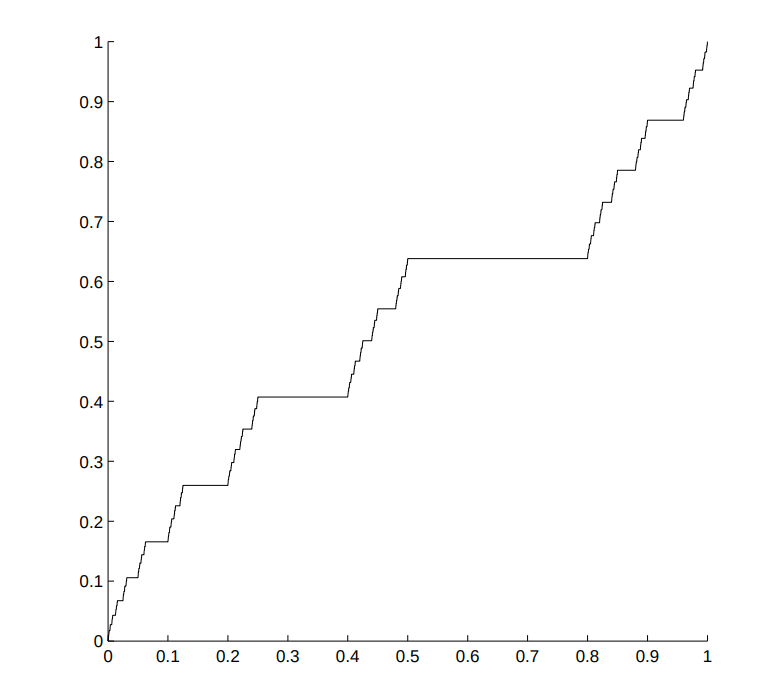
\includegraphics[width=0.7\textwidth]{chapters/chapter4/sections/plots/devils_staircase.png}
\end{center}

\textbf{Properties of the Cantor Function (CDF of \( X \))}\\

(a) It is \textbf{continuous everywhere} across \( [0, 1] \), meaning it has no jump discontinuities.\\
(b) Its derivative is \textbf{zero almost everywhere}, reflecting that the function has a flat slope at almost every point in \( [0, 1] \) except on the Cantor set itself.\\
(c) At points in the Cantor set \( C \), the function increases in value, yet it does so in a manner without a well-defined derivative at those points—illustrating its \textit{staircase} nature without abrupt jumps.\\

The Cantor function thus \textit{climbs} incrementally across the interval \( [0, 1] \) by increasing only at points in the Cantor set. This results in a singular CDF that is entirely smooth yet almost everywhere flat, a distinctive feature setting it apart from typical continuous or discrete distributions.


\begin{exercise}
    Consider a random variable \( X \). Prove that 

\[
P_X(\{y\}) = F_X(y) - \lim_{x \uparrow y} F_X(x).
\]

Furthermore, show that the cumulative distribution function \( F_X \) is continuous at the point \( y \) if and only if the probability that \( X \) takes the value \( y \), denoted as \( P_X(\{y\}) \), is equal to zero.
\end{exercise}

\begin{solution}
Let \( X \) be a random variable, and we want to prove the following statement: 

\[
P_X(\{y\}) = F_X(y) - \lim_{x \uparrow y} F_X(x)
\]

where \( F_X(y) \) denotes the cumulative distribution function (CDF) of \( X \), which is defined as 

\[
F_X(y) = P_X(X \leq y).
\]

To understand the left-hand side, \( P_X(\{y\}) \), we interpret it as the probability that the random variable \( X \) takes on the specific value \( y \). This can be thought of as the measure of the set \( \{y\} \) under the probability measure defined by \( X \).\\

Now, consider the right-hand side of the equation. The term \( F_X(y) \) represents the probability that \( X \) is less than or equal to \( y \). In contrast, \( \lim_{x \uparrow y} F_X(x) \) gives us the probability that \( X \) is less than \( y \) as we approach \( y \) from the left.\\

Thus, we can interpret the difference \( F_X(y) - \lim_{x \uparrow y} F_X(x) \) as the \textit{amount} of probability mass located precisely at \( y \). If there is a non-zero probability that \( X \) equals \( y \), then the CDF will increase at that point, resulting in a positive difference.\\

Next, we will show that \( F_X \) is continuous at \( y \) if and only if \( P_X(\{y\}) = 0 \). \\

(a) \textit{If \( F_X \) is continuous at \( y \)}:
\[
   \text{Then } \lim_{x \uparrow y} F_X(x) = F_X(y).
   \]
   Therefore,
   \[
   P_X(\{y\}) = F_X(y) - \lim_{x \uparrow y} F_X(x) = F_X(y) - F_X(y) = 0.
   \]

(b) \textit{Conversely, if \( P_X(\{y\}) = 0 \)}:
This implies that 
   \[
   F_X(y) - \lim_{x \uparrow y} F_X(x) = 0.
   \]
   Hence,
   \[
   F_X(y) = \lim_{x \uparrow y} F_X(x).
   \]
   This shows that \( F_X \) is continuous at \( y \).\\

In summary, we have established that \( P_X(\{y\}) = F_X(y) - \lim_{x \uparrow y} F_X(x) \), and that \( F_X \) is continuous at \( y \) if and only if \( P_X(\{y\}) = 0 \). \\
\end{solution}


\begin{exercise}
Among the functions given below, identify which are valid cumulative distribution functions (CDFs) and find their corresponding densities. For those that are not valid CDFs, explain the failures.

\textbf{(a) } 
\[
    F(x) = 
    \begin{cases} 
    1 - e^{-x^2} & x \geq 0 \\ 
    0 & x < 0 
    \end{cases}
\]


\textbf{(b) } 
\[
    F(x) = 
    \begin{cases} 
    e^{-\frac{1}{x}} & x > 0 \\ 
    0 & x \leq 0 
    \end{cases}
\]

\textbf{(c) } 
\[
    F(x) = 
    \begin{cases} 
    0 & x \leq 0 \\ 
    \frac{1}{3} & 0 < x \leq 1 \\ 
    2 & x > 1 
    \end{cases}
\]

\end{exercise}

\begin{solution}

\textbf{(a) Analysis:} \\

(a) For \( x < 0 \), \( F(x) = 0 \).\\
(b) For \( x \geq 0 \), as \( x \to 0 \), \( F(0) = 1 - e^{0} = 0 \), and as \( x \to \infty \), \( F(x) \to 1 \).\\
(c) The function is non-decreasing for \( x \geq 0 \) since the derivative \( F'(x) = 2x e^{-x^2} \) is non-negative.\\

Thus, \( F(x) \) is a valid CDF.\\

\textbf{Finding the Density:} The PDF is given by the derivative:
\[
f(x) = \frac{d}{dx}F(x) = 
\begin{cases} 
2x e^{-x^2} & x \geq 0 \\ 
0 & x < 0 
\end{cases}
\]

\textbf{(b) Analysis:} \\

(a) For \( x \leq 0 \), \( F(x) = 0 \).\\
(b) As \( x \to 0^+ \), \( F(x) \to 0 \), but as \( x \to \infty \), \( F(x) \to 1 \).\\
(c) However, the function is non-decreasing for \( x \geq 0 \) because the derivative \( F'(x) = e^{-\frac{1}{x}} \cdot \frac{1}{x^2} \) is always positive.\\

Thus, \( F(x) \) is a valid CDF.\\

\textbf{Finding the Density:} The PDF is given by the derivative:
\[
f(x) = \frac{d}{dx}F(x) = 
\begin{cases} 
    e^{-\frac{1}{x}} \cdot \frac{1}{x^2} & x \geq 0 \\ 
0 & x < 0 
\end{cases}
\]


\textbf{(c) Analysis:} \\

(a) For \( x \leq 0 \), \( F(x) = 0 \).\\
(b) For \( 0 < x \leq 1 \), \( F(x) = \frac{1}{3} \), which is constant and thus non-decreasing.\\
(c) However, for \( x > 1 \), \( F(x) = 2 \), which violates the upper limit condition of a CDF, as \( F(x) \) must approach \( 1 \) as \( x \to \infty \).\\

Thus, \( F(x) \) is not a valid CDF due to exceeding the limit of \( 1 \).\\


\end{solution}


\begin{exercise}
\textbf{Negative Binomial Random Variable.} Consider a sequence of independent Bernoulli trials \(\{X_i\}_{i \in \mathbb{N}}\) with parameter of success \(p \in (0, 1]\). The number of successes in the first \(n\) trials is given by 
\[
Y_n = \sum_{i=1}^{n} X_i.
\]
\(Y_n\) is distributed as Binomial with parameters \(n\) and \(p\). Consider the random variable defined by 
\[
V_k = \min\{n \in \mathbb{N}^+ : Y_n = k\}.
\]
Note that \(V_1\) is distributed as Geometric with parameter \(p\).\\

(a) Give a verbal description of the random variable \(V_k\)\\

(b) Show that the probability mass function of the random variable \(V_k\) is given by 
\[
P(V_k = n) = \binom{n-1}{k-1} p^k (1 - p)^{n-k},
\]
where \(n \in \{k, k + 1, \ldots\}\), we need to consider the conditions under which \(V_k = n\). \\

(c) Argue that the Binomial and Negative Binomial Distributions are inverse to each other in the sense that
\[
Y_n \geq k \Leftrightarrow V_k \leq n,
\]
\end{exercise}

\begin{solution}
\textbf{(a)} A verbal description of the random variable \(V_k\) is as follows: \(V_k\) represents the number of trials required to achieve exactly \(k\) successes in a series of independent Bernoulli trials, where each trial has a success probability of \(p\). In simpler terms, \(V_k\) tells us how many attempts we need to make until we obtain \(k\) successful outcomes.\\

\textbf{(b)} For \(V_k\) to equal \(n\), the following must hold:\\

1. The \(n\)-th trial must result in a success, contributing to the \(k\)-th success.\\
2. Among the first \(n-1\) trials, exactly \(k-1\) must be successes, ensuring that the \(k\)-th success occurs on the \(n\)-th trial.\\

The number of ways to select which \(k-1\) trials out of the first \(n-1\) are successful is given by \(\binom{n-1}{k-1}\). The probability of exactly \(k-1\) successes and \(n-k\) failures in the first \(n-1\) trials is given by \(p^{k-1} (1 - p)^{(n-1) - (k-1)}\) or \(p^{k-1} (1 - p)^{n-k}\). Finally, the \(n\)-th trial must be a success, contributing a factor of \(p\). Therefore, the total probability is:
\[
P(V_k = n) = \binom{n-1}{k-1} p^{k} (1 - p)^{n-k}.
\]

This is known as the Negative Binomial Distribution with parameters \(k\) and \(p\).\\

\textbf{(c)} To argue that the Binomial and Negative Binomial Distributions are inverse to each other in the sense that
\[
Y_n \geq k \Leftrightarrow V_k \leq n,
\]
we interpret these statements as follows:\\

(a) \(Y_n \geq k\) means that in \(n\) trials, we have at least \(k\) successes. This implies that the \(k\)-th success can occur at or before the \(n\)-th trial.\\

(b) \(V_k \leq n\) means that the \(k\)-th success occurs within the first \(n\) trials. This is equivalent to stating that we need \(n\) or fewer trials to achieve \(k\) successes.\\

Thus, the two statements describe the same event: having \(k\) successes in at most \(n\) trials. Consequently, we can conclude that \(Y_n \geq k \Leftrightarrow V_k \leq n\).\\
\end{solution}


\begin{exercise}
    Radioactive decay. Assume that a radioactive sample emits a random number of \(\alpha\) particles in any given hour, and that the number of \(\alpha\) particles emitted in an hour is Poisson distributed with parameter \(\lambda\). Suppose that a faulty Geiger-Muller counter is used to count these particle emissions. In particular, the faulty counter fails to register an emission with probability \(p\), independently of other emissions. \\

    (a) What is the probability that the faulty counter will register exactly \(k\) emissions in an hour? \\
    (b) Given that the faulty counter registered \(k\) emissions in an hour, what is the PMF of the actual number of emissions that happened from the source during that hour?
    \end{exercise}
    
    \begin{solution}
    To solve this problem, we will consider the nature of radioactive decay and the behavior of the faulty counter.\\
    
    First, we know that the number of \(\alpha\) particles emitted in an hour, denoted as \(X\), follows a Poisson distribution with parameter \(\lambda\):
    \[
    P(X = n) = \frac{\lambda^n e^{-\lambda}}{n!}
    \]
    for \(n = 0, 1, 2, \ldots\).\\
    
    The faulty counter registers an emission with probability \(1 - p\) and fails to register it with probability \(p\). Therefore, if \(X\) is the actual number of emissions, the number of emissions registered by the counter, denoted as \(Y\), follows a Binomial distribution:
    \[
    Y | X = n \sim \text{Binomial}(n, 1 - p).
    \]
    
    \textbf{(a)} We want to find the probability that the faulty counter registers exactly \(k\) emissions in an hour, which can be expressed as:
    \[
    P(Y = k) = \sum_{n=k}^{\infty} P(Y = k | X = n) P(X = n).
    \]
    
    The conditional probability \(P(Y = k | X = n)\) for the Binomial distribution is given by:
    \[
    P(Y = k | X = n) = \binom{n}{k} (1 - p)^k p^{n - k}.
    \]
    
    Thus, we have:
    \[
    P(Y = k) = \sum_{n=k}^{\infty} \binom{n}{k} (1 - p)^k p^{n - k} \frac{\lambda^n e^{-\lambda}}{n!}.
    \]
    
    This can be simplified by recognizing that:
    \[
    \binom{n}{k} \frac{1}{n!} = \frac{1}{k!(n-k)!}.
    \]
    
    The expression for \(P(Y = k)\) becomes:
    \[
    P(Y = k) = (1 - p)^k \frac{1}{k!} \sum_{n=k}^{\infty} \frac{(\lambda p)^{n - k}}{(n - k)!} e^{-\lambda}.
    \]
    The inner sum is the series expansion for the exponential function, leading to:
    \[
    \sum_{m=0}^{\infty} \frac{(\lambda p)^m}{m!} = e^{\lambda p}.
    \]
    Therefore, we obtain:
    \[
    P(Y = k) = (1 - p)^k \frac{(\lambda (1 - p))^k e^{-\lambda}}{k!}.
    \]
    
    This shows that \(Y\) also follows a Poisson distribution with parameter \(\lambda (1 - p)\):
    \[
    P(Y = k) = \frac{(\lambda (1 - p))^k e^{-\lambda (1 - p)}}{k!}.
    \]
    
    \textbf{(b)} Next, we need to find the PMF of the actual number of emissions \(X\) given that the counter registered \(k\) emissions:
    \[
    P(X = n | Y = k).
    \]
    Using Bayes' theorem, we can express this as:
    \[
    P(X = n | Y = k) = \frac{P(Y = k | X = n) P(X = n)}{P(Y = k)}.
    \]
    
    Substituting the earlier expressions, we find:
    \[
    P(X = n | Y = k) = \frac{\binom{n}{k} (1 - p)^k p^{n - k} \frac{\lambda^n e^{-\lambda}}{n!}}{P(Y = k)}.
    \]
    
    Given that \(P(Y = k)\) has already been derived, we can substitute this back into our equation. This results in a formula that allows us to compute the conditional probabilities depending on the values of \(n\) and \(k\).\\
    
    In summary, the solution outlines the Poisson nature of emissions and the impact of a faulty counter on the observed counts. 
    \end{solution}
    


\begin{exercise}
Buses arrive at ten minute intervals starting at noon. A man arrives at the bus stop at a random time \(X\) minutes after noon, where \(X\) has the CDF:
\[
F_X(x) =
\begin{cases}
0 & x < 0 \\
\frac{x}{60} & 0 \leq x \leq 60 \\
1 & x > 60.
\end{cases}
\]
What is the probability that he waits less than five minutes for a bus?
\end{exercise}

\begin{solution}
To solve this problem, we first need to understand the situation described. The man arrives at the bus stop at a random time \(X\) uniformly distributed between 0 and 60 minutes after noon. The buses arrive every 10 minutes, which means they arrive at 0, 10, 20, 30, 40, 50, and 60 minutes. The key is to find the probability that the man waits less than 5 minutes for the next bus.\\

The waiting time \(W\) can be calculated based on when he arrives at the bus stop:\\

1. If \(X \in [0, 5)\), the wait time \(W < 5\).\\
2. If \(X \in [5, 10)\), then \(W = 10 - X < 5\) corresponds to \(X > 5\), which means he waits for 0 to 5 minutes.\\
3. This pattern continues for \(X \in [10, 15)\), where he will again have a wait time of less than 5 minutes.\\

More formally, we can analyze the intervals for which \(W < 5\): \(X\) in the intervals \([0, 5)\) and \([10, 15)\), and so on up to \([50, 55)\).\\

To summarize the intervals where \(W < 5\):
\[
X \in [0, 5) \cup [10, 15) \cup [20, 25) \cup [30, 35) \cup [40, 45) \cup [50, 55).
\]

Thus, the total length of intervals where the man waits less than 5 minutes is:
\[
6 \times 5 = 30 \text{ minutes}.
\]

Since \(X\) is uniformly distributed over the interval \([0, 60]\), the probability \(P(W < 5)\) is the ratio of the total length of intervals where he waits less than 5 minutes to the total possible time (60 minutes):
\[
P(W < 5) = \frac{30}{60} = \frac{1}{2}.
\]
\end{solution}


\begin{exercise}
Find the values of \( a \) and \( b \) such that the following function is a valid CDF:
\[
F(x) = 
\begin{cases}
1 - ae^{-x/b} & \text{for } x \geq 0 \\
0 & \text{for } x < 0
\end{cases}
\]
Also, find the values of \( a \) and \( b \) such that the function above corresponds to the CDF of some:
\begin{enumerate}
    \item Continuous Random Variable
    \item Discrete Random Variable
    \item Mixed type Random Variable
\end{enumerate}
\end{exercise}

\begin{solution}
To determine the values of \( a \) and \( b \) that make \( F(x) \) a valid cumulative distribution function (CDF), we need to ensure that:\\

1. \( F(x) \) is non-decreasing.\\
2. \( \lim_{x \to -\infty} F(x) = 0 \) and \( \lim_{x \to \infty} F(x) = 1 \).\\

For the given function \( F(x) \):\\

1. For \( x < 0 \), we have \( F(x) = 0 \), which satisfies the first condition.\\
2. For \( x \geq 0 \), we have \( F(x) = 1 - ae^{-x/b} \).\\

Next, we examine the limits:\\

(a) As \( x \to 0 \):
\[
F(0) = 1 - ae^{0} = 1 - a
\]
To ensure that \( F(0) \) is non-negative, we require:
\[
1 - a \geq 0 \implies a \leq 1
\]

(b) As \( x \to \infty \):
\[
F(x) \to 1 - a \cdot 0 = 1
\]
This is valid if \( a > 0 \) to ensure \( F(x) \) approaches 1 correctly.\\

Thus, from these conditions, we have:
\[
0 < a \leq 1
\]

Next, for \( b \), the exponential function \( e^{-x/b} \) is defined for all \( x \) when \( b > 0 \). Therefore, we must have:
\[
b > 0
\]

In summary, the parameters \( a \) and \( b \) must satisfy:
\[
0 < a \leq 1 \\
b > 0
\]

Now, let’s analyze the types of random variables.\\

(a) \textit{Continuous Random Variable}\\

For \( F(x) \) to represent the CDF of a continuous random variable, the function \( F(x) \) must be strictly increasing. This requires:
\[
a > 0 \quad \text{and} \quad b > 0
\]
Therefore, the same conditions hold.\\

(b) \textit{Discrete Random Variable}\\

For a discrete random variable, \( F(x) \) should have jumps at specific values. In this case, we can choose \( a = 1 \) and \( b \) can be any positive number. Thus:
\[
a = 1, \quad b > 0
\]

(c) \textit{Mixed Random Variable}\\

For a mixed type random variable, \( F(x) \) must be a combination of both continuous and discrete. We can choose \( a < 1 \) and \( b > 0 \). This allows \( F(x) \) to have a continuous component as well as a discrete one at \( x = 0 \). Thus, we can set:
\[
0 < a < 1, \quad b > 0
\]

\end{solution}

    

\begin{exercise}
Let \( X \) be a continuous random variable. Show that \( X \) is memoryless if and only if \( X \) is an exponential random variable.
\end{exercise}

\begin{solution}
To demonstrate that a continuous random variable \( X \) is memoryless if and only if it is an exponential random variable, we first define what it means for \( X \) to be memoryless. A random variable \( X \) is said to be memoryless if it satisfies the following condition for all \( s, t \geq 0 \):

\[
P(X > s + t \mid X > s) = P(X > t).
\]

This equation states that the probability that \( X \) exceeds \( s + t \), given that it has already exceeded \( s \), is the same as the probability that \( X \) exceeds \( t \) alone. \\

(\(\Rightarrow\)) We begin by assuming that \( X \) is memoryless. To show that \( X \) is an exponential random variable, we will derive its cumulative distribution function (CDF) and probability density function (PDF).\\

Let \( F(x) = P(X \leq x) \) be the CDF of \( X \). Consequently, the survival function, which gives the probability that \( X \) exceeds \( x \), is:

\[
S(x) = P(X > x) = 1 - F(x).
\]

Now, using the memoryless property, we have:

\[
P(X > s + t \mid X > s) = \frac{P(X > s + t)}{P(X > s)}.
\]

Using the memoryless condition, we equate this to \( P(X > t) \):

\[
\frac{S(s+t)}{S(s)} = S(t).
\]

Rearranging gives us:

\[
S(s + t) = S(s) S(t).
\]

This functional equation resembles the form of the survival function of an exponential distribution. If we denote \( S(t) = e^{-\lambda t} \) for some \( \lambda > 0 \), then we can verify that:

\[
S(s+t) = e^{-\lambda (s+t)} = e^{-\lambda s} e^{-\lambda t} = S(s) S(t).
\]

Thus, \( S(t) \) takes the form of the exponential survival function, confirming that \( X \) is indeed an exponential random variable.\\

(\(\Leftarrow\)) Conversely, suppose that \( X \) is an exponential random variable with parameter \( \lambda \). The survival function is given by:

\[
S(t) = P(X > t) = e^{-\lambda t}.
\]

We can apply this to check the memoryless property:

\[
P(X > s + t \mid X > s) = \frac{P(X > s+t)}{P(X > s)} = \frac{e^{-\lambda (s+t)}}{e^{-\lambda s}} = e^{-\lambda t} = P(X > t).
\]

Since this holds for all \( s, t \geq 0 \), we conclude that the exponential distribution satisfies the memoryless property.\\

In summary, we have shown that \( X \) is memoryless if and only if \( X \) is an exponential random variable.
\end{solution}

\section{Multiple Random Variables}

We begin by examining multiple random variables defined on a common probability space. Let's focus on two random variables, \(X\) and \(Y\), which are defined on the probability space \((\Omega, \mathcal{F}, P)\). It's crucial to grasp that the values taken by \(X\) and \(Y\) are influenced by the same underlying randomness, represented by \(\omega \in \Omega\).\\

For instance, consider a scenario involving weather on a specific day. We can let the random variable \(X\) represent the temperature of that day, while another random variable \(Y\) denotes the humidity level. Since both \(X\) and \(Y\) are determined by the same outcome, it is natural to expect a certain level of interdependence between them. In this weather example, a higher temperature generally correlates with increased humidity.\\

Say \(X\) and \(Y\) serve as measurable functions from the same probability space to the real numbers. The figure provided represents the pair \((X(\cdot), Y(\cdot))\) as a function mapping \(\Omega\) to \(\mathbb{R}^2\). This representation is particularly significant as it captures the interdependence between \(X\) and \(Y\).\\

A pertinent question arises: is the function \((X(\cdot), Y(\cdot)) : \Omega \to \mathbb{R}^2\) measurable, given that both \(X\) and \(Y\) are measurable functions? To properly address this question, we first need to define the Borel \(\sigma\)-algebra on \(\mathbb{R}^2\). The Borel \(\sigma\)-algebra on \(\mathbb{R}^2\), denoted as \(\mathcal{B}(\mathbb{R}^2)\), is generated by the collection 

\[
\mathcal{P}_{\mathbb{R}^2} = \{ (-\infty, x] \times (-\infty, y] \mid x, y \in \mathbb{R} \}.
\]

Thus, we can express this as 

\[
\mathcal{B}(\mathbb{R}^2) = \sigma(\mathcal{P}_{\mathbb{R}^2}).
\]


\begin{center}
\begin{tikzpicture}[
    >={Stealth[length=6pt]},
    probability space/.style={draw, minimum width=3cm, minimum height=4cm, align=center},
    real line/.style={draw, minimum width=2cm, minimum height=4cm},
    mapping/.style={->, thick, blue},
    point/.style={circle, fill, inner sep=1.5pt},
    label distance=0.5cm
]

% Define the probability space and real lines
\node[probability space] (omega) at (0,0) {};
\node[real line] (R2D) at (9,0) {$\mathbb{R}^2$};

% Add some sample points in probability space
\node[point, label=left:$\omega_1$] (w1) at (0,1) {};
\node[point, label=left:$\omega_2$] (w2) at (0,0) {};
\node[point, label=left:$\omega_3$] (w3) at (0,-1) {};

% Add points on real lines for Temperature and Humidity
\node[point] (x1) at (5,2.5) {};
\node[point] (x2) at (5,2) {};
\node[point] (x3) at (5,1.5) {};

\node[point] (y1) at (6,-1.5) {};
\node[point] (y2) at (6,-2) {};
\node[point] (y3) at (6,-2.5) {};

% Draw vertical lines for Temperature and Humidity
\draw[dashed] (5,-3) -> (5,3);
\draw[dashed] (6,-3) -> (6,3);

% Add points in R^2
\node[point] (xy1) at (8.5,0.5) {};
\node[point] (xy2) at (8.5,0) {};
\node[point] (xy3) at (8.5,-0.5) {};

% Draw mappings
\draw[mapping] (w1) to[bend left=20] node[above, midway] {$X$} (x1);
\draw[mapping] (w2) to[bend left=10] (x2);
\draw[mapping] (w3) to[bend left=0] (x3);

\draw[mapping] (w1) to[bend right=20] node[above, midway] {$Y$} (y1);
\draw[mapping] (w2) to[bend right=10] (y2);
\draw[mapping] (w3) to[bend right=0] (y3);

% Add the combined mapping
\draw[mapping, red] (w1) to[bend left=10]  (xy1);
\draw[mapping, red] (w2) to node[below, below] {$(X,Y)$} (xy2);
\draw[mapping, red] (w3) to[bend right=10] (xy3);

% Add labels and explanations
\node[align=center] at (0,-3) {Sample Space\\$(\Omega, \mathcal{F}, P)$};
\node[align=center] at (6,4) {Temperature\\Values\\$\in \mathcal{B}(\mathbb{R})$};
\node[align=center] at (5,-4) {Humidity\\Values\\$\in \mathcal{B}(\mathbb{R})$};
\node[align=center] at (9,-3) {Joint\\Distribution};
\end{tikzpicture}
\end{center}

\begin{theorem}
    Let \( X \) and \( Y \) be two random variables defined on the probability space \( (\Omega, \mathcal{F}, P) \). The mapping \( (X(\cdot), Y(\cdot)) : \Omega \to \mathbb{R}^2 \) is measurable with respect to \( \mathcal{F} \). This means that the pre-images of Borel sets in \( \mathbb{R}^2 \) under the mapping \( (X(\cdot), Y(\cdot)) \) correspond to events in the probability space.
\end{theorem}

\begin{proof}
    Let \( \mathcal{G} \) be the collection of all subsets of \( \mathbb{R}^2 \) such that their pre-images under \( (X(\cdot), Y(\cdot)) \) are events in \( \mathcal{F} \). To establish the theorem, it suffices to show that the Borel sets \( \mathcal{B}_{\mathbb{R}^2} \) are contained within \( \mathcal{G} \).\\

    The set \( \mathcal{G} \) is a \( \sigma \)-algebra of subsets of \( \mathbb{R}^2 \). This can be easily proved just by following through the definitions.\\

    1. \textbf{Non-emptiness:} \\
   We first show that \( \mathcal{G} \) is non-empty. The empty set \( \emptyset \) belongs to \( \mathcal{G} \) because its pre-image under any function, including \( (X(\cdot), Y(\cdot)) \), is the empty set, which is an event in \( \mathcal{F} \).\\

    2. \textbf{Closed under complements:}\\
    Let \( A \in \mathcal{G} \). By definition, the pre-image of \( A \) under \( (X(\cdot), Y(\cdot)) \) is an event in \( \mathcal{F} \). We denote this pre-image as \( (X,Y)^{-1}(A) \). The complement of \( A \), denoted \( A^c \), has the property that
    \[
    (X,Y)^{-1}(A^c) = \Omega \setminus (X,Y)^{-1}(A),
    \]
    which is also an event in \( \mathcal{F} \) since \( \mathcal{F} \) is a \( \sigma \)-algebra. Thus, \( A^c \in \mathcal{G} \).\\     

    3. \textbf{Closed under countable unions:}\\
    Let \( A_1, A_2, \ldots \) be a countable collection of sets in \( \mathcal{G} \). For each \( n \), the pre-image \( (X,Y)^{-1}(A_n) \) is an event in \( \mathcal{F} \). The pre-image of the union is given by
    \[
    (X,Y)^{-1}\left(\bigcup_{n=1}^{\infty} A_n\right) = \bigcup_{n=1}^{\infty} (X,Y)^{-1}(A_n),
    \]
    and since \( \mathcal{F} \) is a \( \sigma \)-algebra, this union is also an event in \( \mathcal{F} \). Hence, \( \bigcup_{n=1}^{\infty} A_n \in \mathcal{G} \).\\

    Since \( \mathcal{G} \) satisfies all three properties required for a \( \sigma \)-algebra, we conclude that \( \mathcal{G} \) is indeed a \( \sigma \)-algebra.\\

    Next, observe that the sets of the form \( \{ \omega \mid X(\omega) \leq x \} \) and \( \{ \omega \mid Y(\omega) \leq y \} \) belong to \( \mathcal{F} \) for all \( x, y \in \mathbb{R} \) because \( X \) and \( Y \) are random variables.\\

    Given that \( \mathcal{F} \) is a \( \sigma \)-algebra, the intersection of these two sets,
    \[
    \{ \omega \mid X(\omega) \leq x \} \cap \{ \omega \mid Y(\omega) \leq y \},
    \]
    also belongs to \( \mathcal{F} \) for all \( x, y \in \mathbb{R} \).\\

    Consequently, we conclude that 
    \[
    \{ \omega \mid X(\omega) \leq x, Y(\omega) \leq y \} \in \mathcal{F} \text{ for all } x, y \in \mathbb{R}.
    \]
    This implies that the rectangles \( (-\infty, x] \times (-\infty, y] \) belong to \( \mathcal{G} \) for every \( x, y \in \mathbb{R} \) based on the definition of \( \mathcal{G} \).\\

    From this, we can see that the collection of sets formed by all finite unions and complements of sets in \( \mathcal{G} \) will also belong to \( \mathcal{G} \), thus confirming that \( \mathcal{G} \) is indeed a \( \sigma \)-algebra.\\

    Finally, we observe that the collection of rectangles \( (-\infty, x] \times (-\infty, y] \) generates the Borel \( \sigma \)-algebra \( \sigma(\mathcal{P}(\mathbb{R}^2)) \), which contains all Borel sets in \( \mathbb{R}^2 \). Thus, we conclude that \( \mathcal{B}_{\mathbb{R}^2} \subseteq \mathcal{G} \).
\end{proof}

Let us denote the space of events as \(\mathcal{G}\), where the pre-images of Borel sets on \(\mathbb{R}^2\) correspond to events that we can assign probabilities to. This concept leads us to an important definition in probability, known as the \textit{joint probability law.}

\begin{definition}
    The joint probability law for the random variables \(X\) and \(Y\) is defined as follows:

\[
P_{X,Y}(B) = P(\{\omega \in \Omega \mid (X(\omega), Y(\omega)) \in B\}), \quad B \in \mathcal{B}(\mathbb{R}^2),
\]

where \(\mathcal{B}(\mathbb{R}^2)\) denotes the Borel \(\sigma\)-algebra on \(\mathbb{R}^2\). 
\end{definition}

This definition captures the idea that we are interested in the probability of the random vector \((X, Y)\) falling within the set \(B\). To illustrate this with a specific example, consider when we take the set \(B\) to be \((-\infty, x] \times (-\infty, y]\). In this case, the joint probability law can be expressed as:

\[
P_{X,Y}((-\infty, x] \times (-\infty, y]) = P(\{\omega \mid X(\omega) \leq x, Y(\omega) \leq y\}).
\]

Here, we are effectively computing the probability that the random variable \(X\) takes on a value less than or equal to \(x\) and simultaneously, the random variable \(Y\) takes on a value less than or equal to \(y\). This joint perspective allows us to understand the relationship between \(X\) and \(Y\) in a more comprehensive manner.

\subsection{Joint CDF and Its Properties}

\begin{definition}
    Let \( X \) and \( Y \) be two random variables defined on the probability space \( (\Omega, \mathcal{F}, P) \). The joint cumulative distribution function (CDF) of \( X \) and \( Y \) is defined as:

\[
F_{X,Y}(x,y) = P(\{\omega \mid X(\omega) \leq x, Y(\omega) \leq y\}), \quad \forall x,y \in \mathbb{R}.
\]
\end{definition}

In simpler terms, we denote this as \( F_{X,Y}(x,y) = P(X \leq x, Y \leq y) \).\\

\textbf{Properties of Joint CDF}\\

\begin{lemma}
    \textbf{Limits at Infinity.} We have the following limits:
    \[
    \lim_{x \to \infty, y \to \infty} F_{X,Y}(x,y) = 1, \quad \text{and} \quad \lim_{x \to -\infty, y \to -\infty} F_{X,Y}(x,y) = 0.
    \]
\end{lemma}

\begin{proof}
    Consider two unbounded, monotone-increasing sequences \( \{x_n\} \) and \( \{y_n\} \). Then we can express:
   \[
   \lim_{x \to \infty, y \to \infty} F_{X,Y}(x,y) = \lim_{x \to \infty, y \to \infty} P(X \leq x, Y \leq y) = \lim_{n \to \infty} P(X \leq x_n, Y \leq y_n).
   \]
   By using the properties of probability measures:
   \[
   = P\left(\bigcap_{n=1}^{\infty} \{\omega : X(\omega) \leq x_n, Y(\omega) \leq y_n\}\right) = P(\Omega) = 1.
   \]
   The proof for the second part follows a similar line of reasoning and is left as an exercise to the reader. Notably, the order in which we take the limits does not affect the result.
\end{proof}

\begin{lemma}
    \textbf{Monotonicity.} For any \( x_1 \leq x_2 \) and \( y_1 \leq y_2 \), it holds that:
    \[
    F_{X,Y}(x_1, y_1) \leq F_{X,Y}(x_2, y_2).
    \]
\end{lemma}

\begin{proof}
    Given \( x_1 \leq x_2 \) and \( y_1 \leq y_2 \), the event \( \{X \leq x_1, Y \leq y_1\} \) is a subset of the event \( \{X \leq x_2, Y \leq y_2\} \). Therefore, we can conclude:
   \[
   P(X \leq x_1, Y \leq y_1) \leq P(X \leq x_2, Y \leq y_2) \Rightarrow F_{X,Y}(x_1, y_1) \leq F_{X,Y}(x_2, y_2).
   \]
\end{proof}

\begin{lemma}
    \textbf{Continuity from Above.}  The joint CDF \( F_{X,Y} \) is continuous from above:
    \[
    \lim_{u \to 0^+, v \to 0^+} F_{X,Y}(x+u, y+v) = F_{X,Y}(x,y), \quad \forall x,y \in \mathbb{R}.
    \]
\end{lemma}

\begin{proof}
    To show that the joint CDF \( F_{X,Y} \) is continuous from above, we need to demonstrate that:

\[
\lim_{u \to 0^+, v \to 0^+} F_{X,Y}(x+u, y+v) = F_{X,Y}(x,y) \quad \forall x,y \in \mathbb{R}.
\]

consider the expression \( F_{X,Y}(x+u, y+v) \):

\[
F_{X,Y}(x+u, y+v) = P(X \leq x+u, Y \leq y+v).
\]

As \( u \to 0^+ \) and \( v \to 0^+ \), the events \( \{X \leq x+u\} \) and \( \{Y \leq y+v\} \) become increasingly close to the events \( \{X \leq x\} \) and \( \{Y \leq y\} \). \\

Specifically, we have:

\[
\{X \leq x\} \subseteq \{X \leq x+u\} \quad \text{and} \quad \{Y \leq y\} \subseteq \{Y \leq y+v\}.
\]

Therefore, we can express the probability:

\[
P(X \leq x+u, Y \leq y+v) \to P(X \leq x, Y \leq y) \quad \text{as } u \to 0^+ \text{ and } v \to 0^+.
\]

To formalize this, we can use the continuity of probability measures. For any \( \epsilon > 0 \), there exist sufficiently small \( u > 0 \) and \( v > 0 \) such that:

\[
\begin{aligned}
P(X \leq x+u, Y \leq y+v) &= P(X \leq x, Y \leq y) + P((X \leq x+u, Y \leq y+v) \setminus (X \leq x, Y \leq y)) \\
&\leq P(X \leq x, Y \leq y) + P(X > x, Y \leq y) + P(X \leq x, Y > y).
\end{aligned}
\]

As \( u \to 0^+ \) and \( v \to 0^+ \), both \( P(X > x, Y \leq y) \) and \( P(X \leq x, Y > y) \) converge to 0 due to the continuity of the probability measures. Thus, we conclude:

\[
\lim_{u \to 0^+, v \to 0^+} F_{X,Y}(x+u, y+v) = F_{X,Y}(x,y).
\]

\end{proof}

\begin{lemma}
    \textbf{Marginal CDFs.} We also have the property:
    \[
    \lim_{y \to \infty} F_{X,Y}(x,y) = F_X(x).
    \]
\end{lemma}

\begin{proof}
    Let \( \{y_n\} \) be an unbounded, monotone-increasing sequence. Then we can express:
   \[
   \lim_{y \to \infty} F_{X,Y}(x,y) = \lim_{n \to \infty} F_{X,Y}(x,y_n).
   \]
   This leads us to:
   \[
   = \lim_{n \to \infty} P(X \leq x, Y \leq y_n) = P\left(\bigcap_{n=1}^{\infty} \{\omega : X(\omega) \leq x, Y(\omega) \leq y_n\}\right) = P(\{\omega : X(\omega) \leq x\}) = F_X(x),
   \]
   where we again used the continuity of probability measures.
\end{proof}


\section{Independence of Random Variables}

Before we proceed to define the independence of random variables, it is useful to understand the notion of the $\sigma$-algebra generated by a random variable.

\subsection{$\sigma$-algebra Generated by Random Variables}

We first state an elementary result that holds for any arbitrary function.

\begin{lemma}
    Let \(\Omega\) and \(S\) be two non-empty sets, and let \(f: \Omega \to S\) be a function. If \(H\) is a \(\sigma\)-algebra of subsets of \(S\), we aim to show that the collection 

\[
G = \{ A \mid A = f^{-1}(B), B \in H \}
\]

is a \(\sigma\)-algebra of subsets of \(\Omega\).
\end{lemma}

In words, the above lemma states that the collection of pre-images of all the sets belonging to some $\sigma$-algebra on the range of a function, is a $\sigma$-algebra on the domain of that function.\\

Let \((\Omega, \mathcal{F}, P)\) be a probability space, and let \(X: \Omega \to \mathbb{R}\) be a random variable. This random variable \(X\) induces a new probability triple \((\mathbb{R}, \mathcal{B}(\mathbb{R}), P_X)\) on the real line.\\

\begin{definition}
    We define the \(\sigma\)-algebra generated by the random variable \(X\) as follows:

\[
\mathcal{A}(X) = \{E \subseteq \Omega \mid E = X^{-1}(B), \, \forall B \in \mathcal{B}(\mathbb{R})\}.
\]
\end{definition}

This means that \(\mathcal{A}(X)\) consists of all events \(E\) in \(\Omega\) that can be obtained by taking the preimages of Borel sets under the mapping defined by the random variable \(X\).

\begin{lemma}
    \(\mathcal{A}(X) \subseteq \mathcal{F}\), which states that the \(\sigma\)-algebra generated by \(X\) is indeed a sub-\(\sigma\)-algebra of \(\mathcal{F}\).
\end{lemma}

To understand this better, note that each Borel set \(B\) corresponds to an event \(E\) in our probability space. The collection of all such preimages of Borel sets forms the \(\sigma\)-algebra generated by \(X\). Therefore, \(\mathcal{A}(X)\) includes exactly those events whose occurrence is fully determined by the value \(X(\omega)\) we observe.\\

Let's illustrate this concept with two examples:\\

\textbf{Example 1:} Consider a probability space \((\Omega, \mathcal{F}, P)\) and an event \(A \in \mathcal{F}\). Define the indicator random variable for the event \(A\) as \(I_A\). In this case, we can see that 

\[
\mathcal{A}(I_A) = \{\emptyset, A, A^c, \Omega\}.
\]

Thus, \(\mathcal{A}(I_A) \subseteq \mathcal{F}\).\\

\textbf{Example 2:} Let \(([0, 1], \mathcal{B}([0, 1]), \lambda)\) be our probability space, and consider the random variable \(X(\omega) = \omega\) for all \(\omega \in \Omega\). In this scenario, we find that 

\[
\mathcal{A}(X) = \mathcal{F}.
\]

From these examples, we observe that the \(\sigma\)-algebra generated by \(X\) can either be relatively small (as in Example 1) or as large as the entire \(\sigma\)-algebra \(\mathcal{F}\) itself (as in Example 2).

\subsection{Independence of Random Variables}

\begin{definition}
    Two random variables \(X\) and \(Y\) are independent if the \(\sigma\)-algebras generated by these variables, denoted as \(\sigma(X)\) and \(\sigma(Y)\), are independent as well. 
\end{definition}

To clarify, we can think of independence in terms of events defined by these random variables. Specifically, \(X\) and \(Y\) are independent if, for any two Borel sets \(B_1\) and \(B_2\) in \(\mathbb{R}\), the events corresponding to these sets can be expressed as follows:

\[
P\left(\{\omega : X(\omega) \in B_1\} \cap \{\omega : Y(\omega) \in B_2\}\right) = P\left(\{\omega : X(\omega) \in B_1\}\right) \cdot P\left(\{\omega : Y(\omega) \in B_2\}\right)
\]

for all \(B_1, B_2 \in \mathcal{B}(\mathbb{R})\). \\

This means that the probability of both \(X\) falling within \(B_1\) and \(Y\) falling within \(B_2\) simultaneously is simply the product of their individual probabilities of falling within these sets.\\

Additionally, there exists a helpful theorem that characterizes the independence of random variables in terms of their joint cumulative distribution function (CDF). 

\begin{theorem}
\(X\) and \(Y\) are independent if and only if the joint CDF of \(X\) and \(Y\) can be expressed as the product of their individual marginal CDFs.     
\end{theorem}

In mathematical terms, if \(F_{X,Y}(x,y)\) represents the joint CDF of \(X\) and \(Y\), and \(F_X(x)\) and \(F_Y(y)\) denote the marginal CDFs, then \(X\) and \(Y\) are independent if:

\[
F_{X,Y}(x,y) = F_X(x) \cdot F_Y(y)
\]

for all \(x, y\). This equivalence provides a practical method for checking the independence of random variables based on their distribution functions.

\begin{proof}
    To prove this theorem, we need to establish both the necessary and sufficient conditions for the independence of random variables \(X\) and \(Y\).\\

    \textbf{Proof of the necessary condition:} \\

Assume that \(X\) and \(Y\) are independent random variables. By the definition of independence, for any two Borel sets \(B_1 \in \mathcal{B}(\mathbb{R})\) and \(B_2 \in \mathcal{B}(\mathbb{R})\), the events \( \{ \omega \mid X(\omega) \in B_1 \} \) and \( \{ \omega \mid Y(\omega) \in B_2 \} \) are independent. This means that:

\[
P(X \in B_1, Y \in B_2) = P(X \in B_1) P(Y \in B_2).
\]

From the definition of the joint cumulative distribution function (CDF), we have:

\[
P(X \in B_1, Y \in B_2) = P_{X,Y}(B_1 \times B_2).
\]

Thus, we can write:

\[
P_{X,Y}(B_1 \times B_2) = P(X \in B_1) P(Y \in B_2).
\]

This holds for all Borel sets in \(\mathbb{R}\). \\

Now, we specifically choose the sets \(B_1 = (-\infty, x]\) and \(B_2 = (-\infty, y]\). Consequently, we obtain:

\[
F_{X,Y}(x, y) = P(X \leq x, Y \leq y) = P(X \leq x) P(Y \leq y) = F_X(x) F_Y(y),
\]

for all \(x, y \in \mathbb{R}\). This completes the proof of the necessary condition.\\

\textbf{Proof of the sufficient condition:}\\

Now, we will prove the sufficiency part. Assume that the joint cumulative distribution function (CDF) of \(X\) and \(Y\) can be expressed as:

\[
F_{X,Y}(x, y) = F_X(x) F_Y(y), \quad \forall x, y \in \mathbb{R}.
\]

To show that \(X\) and \(Y\) are independent, we need to demonstrate that for any Borel sets \(B_1\) and \(B_2\), the events defined by these sets are independent.\\

Using the property of joint CDFs, we can express the probability of the joint event as follows:

\[
P(X \in B_1, Y \in B_2) = P(X \leq x_1, Y \leq y_1) \quad \text{for } (x_1, y_1) \in B_1 \times B_2.
\]

Using the given expression for the joint CDF, we have:

\[
P(X \in B_1, Y \in B_2) = F_{X,Y}(x_1, y_1) = F_X(x_1) F_Y(y_1).
\]

Now, we also know:

\[
P(X \in B_1) = F_X(x_1) \quad \text{and} \quad P(Y \in B_2) = F_Y(y_1).
\]

Thus, we can write:

\[
P(X \in B_1, Y \in B_2) = P(X \in B_1) P(Y \in B_2).
\]

Since this holds for any arbitrary Borel sets \(B_1\) and \(B_2\), we conclude that the events \( \{X \in B_1\} \) and \( \{Y \in B_2\} \) are independent. \\

Therefore, we have established that if the joint CDF can be expressed as the product of the marginal CDFs, then \(X\) and \(Y\) are indeed independent.

\end{proof}

Let's extend our results to a general $n$ random variables. 

\begin{definition}    
Random variables \(X_1, X_2, \ldots, X_n\) are independent if the collections of events associated with these variables, represented by their \(\sigma\)-algebras \(\sigma(X_1), \sigma(X_2), \ldots, \sigma(X_n)\), are independent.
\end{definition}

This means that for any measurable sets \(B_i \in \mathcal{B}(\mathbb{R})\) for \(1 \leq i \leq n\), the joint probability can be expressed as the product of their individual probabilities. Mathematically, this is written as:

\[
P(X_1 \in B_1, X_2 \in B_2, \ldots, X_n \in B_n) = \prod_{i=1}^{n} P(X_i \in B_i).
\]

In simpler terms, knowing the outcome of one random variable does not give us any information about the others when they are independent.\\

Furthermore, we can characterize the independence of these random variables in terms of their cumulative distribution functions (CDFs). 

\begin{theorem}
    The random variables \(X_1, X_2, \ldots, X_n\) are independent if and only if their joint CDF can be expressed as the product of their individual CDFs. 

\[
F_{X_1, X_2, \ldots, X_n}(x_1, x_2, \ldots, x_n) = \prod_{i=1}^{n} F_{X_i}(x_i).
\]
\end{theorem}

This theorem emphasizes that the joint distribution function of the independent random variables is completely determined by their individual distribution functions. In essence, this means that the behavior of the entire system of random variables can be understood by examining each variable independently, highlighting the fundamental nature of independence in probability.

\begin{definition}
A family of random variables \(\{X_i\}_{i \in I}\) as independent if the collections of events associated with these random variables, represented by their \(\sigma\)-algebras \(\{\sigma(X_i) : i \in I\}\), are independent. \\

This means that for any finite selection of indices \(i_1, i_2, \ldots, i_n\) from the index set \(I\), the joint probability of the corresponding random variables can be expressed as the product of their individual probabilities. Mathematically, for any sets \(B_{i_j} \in \mathcal{B}(\mathbb{R})\) for \(j = 1, 2, \ldots, n\), we have:

\[
P(X_{i_1} \in B_{i_1}, X_{i_2} \in B_{i_2}, \ldots, X_{i_n} \in B_{i_n}) = \prod_{j=1}^{n} P(X_{i_j} \in B_{i_j}).
\]
\end{definition}


In simpler words, the independence of the family of random variables implies that knowing the value of one variable provides no information about the values of the others. Thus, the concept of independence can be generalized beyond a finite number of random variables to an arbitrary family indexed by a set \(I\), reinforcing the idea that the individual behavior of each variable remains unaffected by the others in the family.
\section{Conditional Distributions and Joint Continuity}

\subsection{Joint PMF of Discrete Random Variables}

If \( X \) and \( Y \) are discrete random variables, the range of the mapping \( (X(\cdot), Y(\cdot)) \) forms a countable subset of \( \mathbb{R}^2 \). This arises from the fact that the Cartesian product of two countable sets is also countable. To clarify, a set is considered countable if it can be put into a one-to-one correspondence with the natural numbers. Therefore, since both \( X \) and \( Y \) take on countably many values, their combined behavior represented by \( (X, Y) \) will also be countable, thus making \( (X(\cdot), Y(\cdot)) \) a discrete random variable on \( \mathbb{R}^2 \).\\

It's important to note that we cannot make the same assertion when \( X \) and \( Y \) are continuous random variables. In such cases, even if \( X \) and \( Y \) are each continuous on their own, they may not be jointly continuous. Refer subsection 4.5.3 for this. \\

The joint probability mass function (pmf) of the discrete random variables \( X \) and \( Y \) is given by:

\[
p_{X,Y}(x, y) = P(X = x, Y = y), \quad x, y \in \mathbb{R}.
\]

This joint pmf plays a crucial role in defining the joint distribution of \( X \) and \( Y \). Specifically, for any Borel set \( B \in \mathcal{B}_{\mathbb{R}^2} \), the probability that the random vector \( (X, Y) \) falls within the set \( B \) is given by:

\[
P_{X,Y}(B) = \sum_{(x,y) \in B} p_{X,Y}(x, y).
\]

This equation shows that the joint pmf allows us to calculate probabilities associated with any region in the plane defined by the variables \( X \) and \( Y \).


\subsection{Conditional PMF of Discrete Random Variables}

Now, we define the conditional probability mass function (pmf) for discrete random variables.\\

\begin{definition}
    Let \(X\) and \(Y\) be discrete random variables defined on the probability space \((\Omega, \mathcal{F}, P)\). The conditional probability of \(X\) given \(Y\) is defined as:

\[
p_{X|Y}(x|y) = P(X = x | Y = y) = \frac{P(X = x, Y = y)}{P(Y = y)} = \frac{p_{X,Y}(x, y)}{p_Y(y)}
\]

where \(p_Y(y) > 0\).
\end{definition}

The following theorem describes the concept of independence for discrete random variables in terms of the conditional pmf.

\begin{theorem}
    The following statements are equivalent for discrete random variables \(X\) and \(Y\):\\

1. \(X\) and \(Y\) are independent.\\
2. For all \(x, y \in \mathbb{R}\), the events \(\{X = x\}\) and \(\{Y = y\}\) are independent.\\
3. For all \(x, y \in \mathbb{R}\), \(P_{X,Y}(x, y) = P_X(x)P_Y(y)\).\\
4. For all \(x, y \in \mathbb{R}\) such that \(p_Y(y) > 0\), \(p_{X|Y}(x|y) = p_X(x)\).
`'
\end{theorem}

\begin{proof}
    
The equivalences (2) $\Leftrightarrow$ (3) and (3) $\Leftrightarrow$ (4) follow directly from the definitions of independence and the conditional pmf. \\

Now, let us prove the equivalence between (1) and (3):\\

\textbf{(1) implies (3):} If \(X\) and \(Y\) are independent, then the joint probability of \(X\) and \(Y\) can be expressed as:

\[
P(X \in B_1, Y \in B_2) = P(X \in B_1) P(Y \in B_2).
\]

Now, let \(B_1 = \{x\}\) and \(B_2 = \{y\}\). Therefore, we have:

\[
P(X = x, Y = y) = P(X = x) P(Y = y).
\]

This establishes statement (3).\\

\textbf{(3) implies (1):} Given that \(P(X \in B_1, Y \in B_2) = P_{X,Y}(x,y)\), we can write:

\[
P(X \in B_1, Y \in B_2) = \sum_{x \in B_1} \sum_{y \in B_2} p_{X,Y}(x, y).
\]

Using statement (3), we substitute to obtain:

\[
\sum_{x \in B_1} \sum_{y \in B_2} P_X(x) P_Y(y) = \sum_{x \in B_1} P_X(x) \sum_{y \in B_2} P_Y(y) = P(X \in B_1) P(Y \in B_2).
\]

This confirms statement (1). Thus, we have shown that the statements are equivalent.
\end{proof}

\subsection{Joint PMF of Continuous Random Variables}

\begin{definition}
    Two random variables \( X \) and \( Y \) are termed \textit{jointly continuous} if their joint probability distribution, denoted \( P_{X,Y} \), is absolutely continuous with respect to the Lebesgue measure on \( \mathbb{R}^2 \). This means that for every Borel set \( N \subset \mathbb{R}^2 \) with Lebesgue measure zero, we have:
    \[
    P((X, Y) \in N) = 0.
    \]
\end{definition}

In simple terms, this ensures that there is no \textit{mass} of probability concentrated on any set of points with zero area in \( \mathbb{R}^2 \). For \( X \) and \( Y \) to be jointly continuous, their probability distribution must spread smoothly over regions in \( \mathbb{R}^2 \), without \textit{spikes} or \textit{isolated points.}\\

The \textit{Radon-Nikodym Theorem} gives us a more practical tool here. 

\begin{theorem}
    \( X \) and \( Y \) are jointly continuous random variables if and only if there exists a measurable function \( f_{X,Y} : \mathbb{R}^2 \to [0, \infty) \), called the \textit{joint probability density function} (pdf), such that for any region \( B \subset \mathbb{R}^2 \),
    \[
    P((X, Y) \in B) = \int_{B} f_{X,Y}(u, v) \, d\lambda(u, v),
    \]
    where \( \lambda \) represents the Lebesgue measure on \( \mathbb{R}^2 \).
\end{theorem}

\textbf{Implication of Joint Continuity}: To express this in a familiar form, let’s examine the probability that \( X \) and \( Y \) fall within certain ranges. For \( B = (-\infty, x] \times (-\infty, y] \), this probability becomes:
\[
F_{X,Y}(x, y) = P(X \leq x, Y \leq y) = \int_{-\infty}^{x} \int_{-\infty}^{y} f_{X,Y}(u, v) \, dv \, du,
\]
where \( F_{X,Y}(x, y) \) is the \textit{joint cumulative distribution function} (cdf), and \( f_{X,Y}(x, y) \) is the \textit{joint pdf}. \\

Thus, the joint pdf \( f_{X,Y}(x, y) \) provides a complete description of the joint behavior of \( X \) and \( Y \). This means that knowing \( f_{X,Y}(x, y) \) allows us to compute the probabilities for any event involving \( X \) and \( Y \) over regions in \( \mathbb{R}^2 \). \\

\begin{lemma}
    If \( X \) is continuous and \( Y \) is continuous, then \((X, Y)\) need not be jointly continuous.
\end{lemma}

We won't formally prove this lemma, but we will provide an example that confirms that this is true. 

\begin{example}
    Suppose \( X \sim N(0, 1) \), meaning that \( X \) is a standard normal random variable with mean \( 0 \) and variance \( 1 \), and \( Y = 2X \). So, \( Y \) will have a mean of \( 0 \) and a variance of \( 4 \), which we can verify by noting that
\[
Y \sim N(0, 4).
\]

Even though both \( X \) and \( Y \) are continuous random variables, we need to examine if they form a jointly continuous pair when taken together as the random vector \( (X, Y) \).\\

A pair of random variables \( (X, Y) \) is considered jointly continuous if there exists a joint probability density function \( f_{X,Y}(x, y) \) over the entire \( \mathbb{R}^2 \) space, such that for any subset \( A \subset \mathbb{R}^2 \),
\[
P((X, Y) \in A) = \iint_A f_{X,Y}(x, y) \, dx \, dy.
\]

Notice that \( Y = 2X \) directly ties \( Y \) to \( X \). This means \( Y \) is perfectly linearly dependent on \( X \), implying that \( (X, Y) \) does not vary freely across the \( \mathbb{R}^2 \) plane. Instead, the values of \( (X, Y) \) are restricted to a specific line, namely \( y = 2x \). Since \( Y = 2X \), the pair \( (X, Y) \) essentially lies along the line \( y = 2x \) in the \( \mathbb{R}^2 \) plane. Consequently, the joint probability measure of \( (X, Y) \) is concentrated along this line rather than spread across two dimensions.\\ 

In terms of probability density, this restriction means that there does not exist a two-dimensional joint density \( f_{X,Y}(x, y) \) over the entire \( \mathbb{R}^2 \) space, because we cannot assign probabilities over regions in \( \mathbb{R}^2 \) outside this line. Any density that would describe \( (X, Y) \) is confined to one dimension along \( y = 2x \).\\


Thus, although \( X \) and \( Y \) are individually continuous, \( (X, Y) \) as a pair does not possess joint continuity in two dimensions.
\end{example}

\begin{lemma}
    When \( X \) and \( Y \) are jointly continuous random variables, their marginal distributions are also continuous. To understand why, let’s examine the probability that \( X \leq x \) and \( Y \leq y \):
\[
P(X \leq x, Y \leq y) = \int_{-\infty}^{x} \int_{-\infty}^{y} f_{X,Y}(u, v) \, dv \, du
\]
\end{lemma}


Now, we want to find the marginal distribution of \( X \). The marginal probability \( P(X \leq x) \) is obtained by integrating over all possible values of \( Y \):

\[
P(X \leq x) = \int_{-\infty}^{x} \left( \int_{-\infty}^{\infty} f_{X,Y}(u, v) \, dv \right) du = \int_{-\infty}^{x} f_X(u) \, du
\]

Here, the expression inside the parentheses,

\[
\int_{-\infty}^{\infty} f_{X,Y}(u, v) \, dv,
\]

produces a function of \( u \) which is non-negative and measurable. This function represents the density of \( X \), which we denote as \( f_X(u) \). \\

Thus, we can write:

\[
f_X(u) = \int_{-\infty}^{\infty} f_{X,Y}(u, v) \, dv
\]

This shows that \( X \) has a continuous marginal distribution with \( f_X \) as its probability density function (pdf). Since \( f_X(u) \) is derived as an integral over a non-negative function \( f_{X,Y}(u, v) \), it ensures that \( f_X \) itself is also non-negative and measurable.\\

A similar argument applies to the marginal pdf of \( Y \), confirming that both \( X \) and \( Y \) are indeed continuous. This continuity of the marginals follows directly from the joint continuity of \( X \) and \( Y \), as we have shown through their integrals.

\begin{definition}
    \textbf{Independence of Joint Continuous Random Variables.} For two random variables \( X \) and \( Y \), we say they are \textbf{independent} if and only if their joint distribution function \( F_{X,Y}(x, y) \) can be written as the product of their marginal distribution functions. In other words, 

    \[
    F_{X,Y}(x, y) = F_X(x) F_Y(y) \quad \forall x, y \in \mathbb{R}.
    \]
\end{definition}

Now, let's apply this definition to a specific case: when \( X \) and \( Y \) are \textbf{jointly continuous} random variables. For continuous variables, we express independence in terms of their probability density functions. That is, we integrate the joint density function \( f_{X,Y}(x, y) \) over the range \((-\infty, x]\) and \((-\infty, y]\):

\[
\int_{-\infty}^{x} \int_{-\infty}^{y} f_{X,Y}(u, v) \, dv \, du = 
\left( \int_{-\infty}^{x} f_X(u) \, du \right) \left( \int_{-\infty}^{y} f_Y(v) \, dv \right).
\]

Expanding this, we see that independence requires

\[
\int_{-\infty}^{x} \int_{-\infty}^{y} f_{X,Y}(u, v) \, dv \, du = \int_{-\infty}^{x} \int_{-\infty}^{y} f_X(u) f_Y(v) \, dv \, du.
\]

Since this equality holds for \textit{all} values of \( x \) and \( y \), we can conclude that the two integrands themselves must be equal almost everywhere. Therefore,

\[
f_{X,Y}(x, y) = f_X(x) f_Y(y) \quad \forall x, y \in \mathbb{R},
\]

except possibly on a subset of \( \mathbb{R}^2 \) with Lebesgue measure zero. This condition—that the joint density factorizes as the product of the marginal densities—is both a \textbf{necessary and sufficient condition} for the independence of two jointly continuous random variables.

\subsection{Conditional PDF of Continuous Random Variables}

To define the conditional cumulative distribution function (CDF) \( F_{X|Y}(x | y) \approx P(X \leq x | Y = y) \), we face a technical challenge: the event \( \{ Y = y \} \) has probability zero for any specific \( y \) when \( Y \) is a continuous random variable. This zero-probability event makes a direct conditional probability definition problematic.\\

To resolve this, we approximate by conditioning on \( Y \) taking values within a small interval \( (y, y + \epsilon) \), where \( \epsilon > 0 \). We then examine what happens as \( \epsilon \) approaches zero. This approach leads to a motivating derivation for defining the conditional probability density function (pdf) in the jointly continuous case.\\

The conditional CDF of \( X \), given that \( Y \) is \textit{close to \( y \),} can be approximated by:
\[
F_{X|Y}(x | y) = P(X \leq x \mid y \leq Y \leq y + \epsilon) \quad \text{(for small } \epsilon \text{)}.
\]
This probability can be rewritten in terms of joint and marginal probabilities as:
\[
F_{X|Y}(x | y) = \frac{P(\{ X \leq x \} \cap \{ y \leq Y \leq y + \epsilon \})}{P(y \leq Y \leq y + \epsilon)}.
\]
To express this in terms of CDFs, we observe that:
\[
F_{X|Y}(x | y) = \frac{F_{X,Y}(x, y + \epsilon) - F_{X,Y}(x, y)}{F_{Y}(y + \epsilon) - F_{Y}(y)}.
\]
Now, dividing the numerator and denominator by \( \epsilon \), we obtain:
\[
F_{X|Y}(x | y) = \frac{\frac{F_{X,Y}(x, y + \epsilon) - F_{X,Y}(x, y)}{\epsilon}}{\frac{F_{Y}(y + \epsilon) - F_{Y}(y)}{\epsilon}}.
\]
As \( \epsilon \to 0 \), the right-hand side of this expression resembles the form of a derivative. Specifically, it suggests:
\[
F_{X|Y}(x | y) = \frac{\frac{\partial}{\partial y} F_{X,Y}(x, y)}{\frac{d}{d y} F_{Y}(y)}.
\]
This expression provides a foundation for defining the conditional CDF and, by extension, the conditional PDF.


\begin{definition}
    The \textbf{conditional cumulative distribution function} (CDF) of a random variable \( X \) given \( Y = y \) is a way to accumulate probability up to a certain point \( x \), while taking into account the information provided by \( Y = y \). It is defined as:
   \[
   F_{X|Y}(x | y) = \int_{-\infty}^{x} \frac{f_{X,Y}(u, y)}{f_Y(y)} \, du,
   \]
   where \( f_{X,Y}(u, y) \) is the joint probability density function (pdf) of \( X \) and \( Y \), and \( f_Y(y) \) is the marginal pdf of \( Y \). 
\end{definition}

Note that this expression is valid as long as \( f_Y(y) > 0 \), since we cannot condition on an impossible or zero-probability event.

\begin{definition}
    The \textbf{conditional probability density function} (pdf) of \( X \) given \( Y = y \) tells us the probability density of \( X \) at a particular point \( x \), assuming \( Y = y \). It is defined as:
    \[
    f_{X|Y}(x | y) = \frac{f_{X,Y}(x, y)}{f_Y(y)},
    \]
    again, assuming \( f_Y(y) > 0 \).
\end{definition}

This expression gives us a way to interpret \( X \) as a function of the specific value \( y \) of \( Y \), concentrating our attention on the values \( X \) takes when \( Y = y \).

\begin{definition}
    Suppose we have an event \( A \) that belongs to the Borel \(\sigma\)-algebra \( \mathcal{B}(\mathbb{R}) \) (denoted \( A \in \mathcal{B}(\mathbb{R}) \), the collection of all Borel subsets of \( \mathbb{R} \)). The \textbf{conditional probability} of the event \( A \) given \( Y = y \) is defined as:
   \[
   P(X \in A | Y = y) = \int_{A} f_{X|Y}(v | y) \, dv = \int_{-\infty}^{\infty} \mathbb{I}_A(v) f_{X|Y}(v | y) \, dv,
   \]
   where \( \mathbb{I}_A(v) \) is the indicator function for the set \( A \), which is 1 if \( v \in A \) and 0 otherwise.
\end{definition}

This integral sums up the conditional pdf \( f_{X|Y}(v | y) \) over the region defined by \( A \), thereby giving the probability that \( X \) lies in \( A \), under the condition that \( Y = y \).


\begin{exercise}
Consider random variables \( X \) and \( Y \) with a joint continuous distribution defined over a triangular region with vertices at points \( (0, 0) \), \( (0, 2) \), and \( (1, 0) \). The joint probability density function is given by:
\[
f_{X,Y}(x, y) = 1
\]
for \((x, y)\) within the triangular region. Find the marginal distributions \( f_X(x) \) and \( f_Y(y) \), and the conditional distributions \( f_{Y|X}(y|x) \) and \( f_{X|Y}(x|y) \).\\

\begin{center}
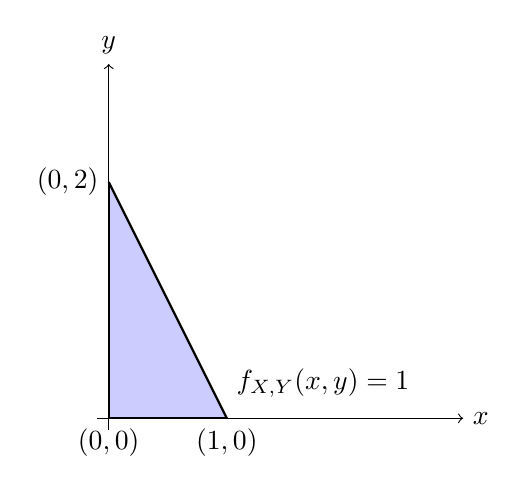
\begin{tikzpicture}[scale=1.5]
    % Draw axes
    \draw[->] (-0.1, 0) -- (3, 0) node[right] {$x$};
    \draw[->] (0, -0.1) -- (0, 3) node[above] {$y$};

    % Draw the triangular region
    \fill[blue!20] (0, 0) -- (0, 2) -- (1, 0) -- cycle;

    % Draw the edges of the triangle
    \draw[thick] (0, 0) -- (0, 2) node[above,left] {$(0, 2)$};
    \draw[thick] (0, 2) -- (1, 0) node[below, below] {$(1, 0)$};
    \draw[thick] (1, 0) -- (0, 0) node[left,below] {$(0, 0)$};

    % Add a label for the area
    \node[below right] at (1, 0.5) {$f_{X,Y}(x,y) = 1$};
\end{tikzpicture}
\end{center}

\end{exercise}

\begin{solution}
The region where \( f_{X,Y}(x, y) = 1 \) is the triangle with vertices \( (0, 0) \), \( (0, 2) \), and \( (1, 0) \). The line connecting \( (0, 2) \) and \( (1, 0) \) has the equation:
    \[
    y = 2 - 2x
    \]
    Therefore, the joint distribution \( f_{X,Y}(x, y) = 1 \) is defined for \( 0 \leq x \leq 1 \) and \( 0 \leq y \leq 2 - 2x \).\\

To ensure \( f_{X,Y}(x, y) = 1 \) is a valid probability density function, we need:
    \[
    \int_0^1 \int_0^{2 - 2x} 1 \, dy \, dx = 1
    \]
    Compute this integral:
    \[
    \int_0^1 \int_0^{2 - 2x} 1 \, dy \, dx = \int_0^1 (2 - 2x) \, dx = \int_0^1 2 - 2x \, dx = \left[ 2x - x^2 \right]_0^1 = 2 - 1 = 1
    \]
    Thus, \( f_{X,Y}(x, y) = 1 \) is indeed normalized.\\

To find \( f_X(x) \), integrate \( f_{X,Y}(x, y) \) over \( y \):
    \[
    f_X(x) = \int_0^{2 - 2x} 1 \, dy = 2 - 2x
    \]
    for \( 0 \leq x \leq 1 \).\\

To find \( f_Y(y) \), integrate \( f_{X,Y}(x, y) \) over \( x \). Note that for a given \( y \), \( x \) ranges from \( 0 \) to \( 1 - \frac{y}{2} \) (from the line equation rearranged):
    \[
    f_Y(y) = \int_0^{1 - \frac{y}{2}} 1 \, dx = 1 - \frac{y}{2}
    \]
    for \( 0 \leq y \leq 2 \).\\

The conditional distribution \( f_{Y|X}(y|x) \) is given by:
    \[
    f_{Y|X}(y|x) = \frac{f_{X,Y}(x, y)}{f_X(x)} = \frac{1}{2 - 2x}
    \]
    for \( 0 \leq y \leq 2 - 2x \).\\

The conditional distribution \( f_{X|Y}(x|y) \) is given by:
    \[
    f_{X|Y}(x|y) = \frac{f_{X,Y}(x, y)}{f_Y(y)} = \frac{1}{1 - \frac{y}{2}}
    \]
    for \( 0 \leq x \leq 1 - \frac{y}{2} \).

\end{solution}


\begin{exercise}
Two persons X and Y live in cities A and B but work in cities B and A respectively. Every morning they start for work at a uniformly random time between 9 am and 10 am independent of each other. Both of them travel at the same constant speed and it takes 20 minutes to reach the other city. What is the probability that X and Y meet each other on their way to work?
\end{exercise}

\begin{solution}
Let \( T_X \) and \( T_Y \) be the times at which persons X and Y leave their respective cities. Both \( T_X \) and \( T_Y \) are uniformly distributed over the interval \([0, 60]\) minutes, where 0 corresponds to 9:00 am and 60 corresponds to 10:00 am. The travel time for both X and Y is 20 minutes. Therefore X will reach city B at \( T_X + 20 \) minutes and Y will reach city A at \( T_Y + 20 \) minutes.\\

For X and Y to meet, they must be on the road at the same time. This occurs if X leaves before Y arrives in city A, and Y leaves before X arrives in city B, which can be expressed as:
\[
T_X + 20 > T_Y \quad \text{and} \quad T_Y + 20 > T_X.
\]

These inequalities can be rearranged to:
\[
T_Y < T_X + 20 \quad \text{and} \quad T_X < T_Y + 20.
\]

This forms a square on the coordinate plane where the side length is 60 minutes (the range of the departure times). 

\begin{center}
    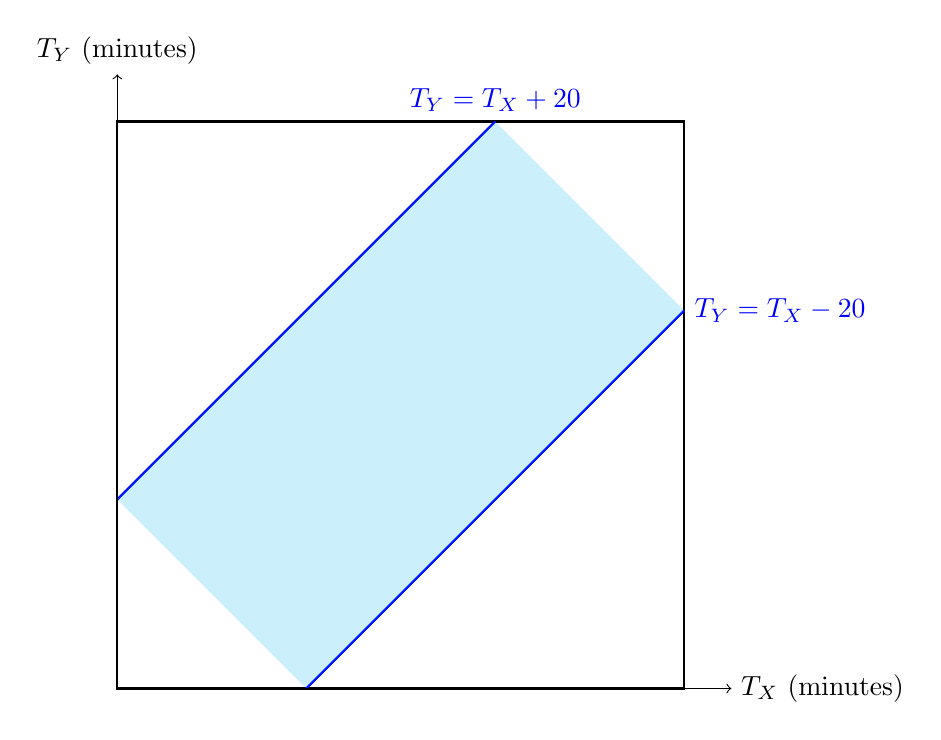
\begin{tikzpicture}[scale=0.12]
        % Draw the square representing all possible combinations of T_X and T_Y
        \draw[thick] (0,0) rectangle (60,60);
        
        % Draw the lines for the conditions T_Y < T_X + 20 and T_Y > T_X - 20
        \draw[blue, thick, domain=0:40] plot (\x, {\x + 20}) node[above] {$T_Y = T_X + 20$};
        \draw[blue, thick, domain=20:60] plot (\x, {\x - 20}) node[right] {$T_Y = T_X - 20$};
        
        % Draw the area of meeting
        \fill[cyan, opacity=0.2] (0,20) -- (40,60) -- (60,40) -- (20,0) -- cycle;
    
        % Label the axes
        \draw[->] (0,0) -- (0,65) node[above] {$T_Y$ (minutes)};
        \draw[->] (0,0) -- (65,0) node[right] {$T_X$ (minutes)};
    \end{tikzpicture}
\end{center}

1. The area of the square representing all possible combinations of departure times is:
\[
A_{\text{total}} = 60 \times 60 = 3600.
\]

2. The region where they meet can be represented by the inequalities. Graphically, this creates a band around the line \( T_Y = T_X \) within the square. The bounds for \( T_Y \) are:
\[
T_Y < T_X + 20 \quad \text{and} \quad T_Y > T_X - 20.
\]

3. This forms a parallelogram with vertices at (0, 20), (40, 60), (60, 40), and (20, 0). The area of this meeting region can be calculated by:
\[
A_{\text{meet}} = 60^2 - 4 \times \frac{1}{2} \times 20 \times 20 = 3600 - 800 = 2800.
\]

4. Finally, the probability \( P \) that X and Y meet each other on their way to work is given by the ratio of the area where they meet to the total area:
\[
P = \frac{A_{\text{meet}}}{A_{\text{total}}} = \frac{2800}{3600} = \frac{7}{9}.
\]

\end{solution}


\begin{exercise}
Data is taken on the height and shoe size of a sample of MIT students. Height (X) is coded by 3 values: 1 (short), 2 (average), 3 (tall) and Shoe size (Y) is coded by 3 values: 1 (small), 2 (average), 3 (large). The joint counts are given in the following table:

\[
\begin{array}{c|c|c|c}
& Y=1 & Y=2 & Y=3 \\
\hline
X=1 & 234 & 225 & 84 \\
\hline
X=2 & 180 & 453 & 161 \\
\hline
X=3 & 39 & 192 & 157 \\
\end{array}
\]

(a) Find the joint and marginal pmf of X and Y. \\
(b) Are X and Y independent? Discuss in detail.
\end{exercise}

\begin{solution}
To solve the problem, we start by calculating the joint probability mass function (pmf) of \(X\) and \(Y\) from the given joint counts.\\

Let \(N\) be the total number of observations, which is the sum of all joint counts:

\[
N = 234 + 225 + 84 + 180 + 453 + 161 + 39 + 192 + 157 = 1260.
\]

The joint probabilities \(P(X=x, Y=y)\) can be calculated as follows:

\[
\renewcommand{\arraystretch}{1.5} % Adjust the value as needed
\begin{array}{c|c|c|c}
& Y=1 & Y=2 & Y=3 \\
\hline
X=1 & \frac{234}{1260} & \frac{225}{1260} & \frac{84}{1260} \\
\hline
X=2 & \frac{180}{1260} & \frac{453}{1260} & \frac{161}{1260} \\
\hline
X=3 & \frac{39}{1260} & \frac{192}{1260} & \frac{157}{1260} \\
\end{array}
\]

Next, we find the marginal pmfs \(P(X = x)\) and \(P(Y = y)\).

For \(P(X = x)\):
\[
\begin{aligned}
P(X = 1) & = P(X = 1, Y = 1) + P(X = 1, Y = 2) + P(X = 1, Y = 3) \\
          & = \frac{234 + 225 + 84}{1260} = \frac{543}{1260} = 0.4300, \\
P(X = 2) & = P(X = 2, Y = 1) + P(X = 2, Y = 2) + P(X = 2, Y = 3) \\
          & = \frac{180 + 453 + 161}{1260} = \frac{794}{1260} = 0.6286, \\
P(X = 3) & = P(X = 3, Y = 1) + P(X = 3, Y = 2) + P(X = 3, Y = 3) \\
          & = \frac{39 + 192 + 157}{1260} = \frac{388}{1260} = 0.3080.
\end{aligned}
\]

For \(P(Y = y)\):
\[
\begin{aligned}
P(Y = 1) & = P(X = 1, Y = 1) + P(X = 2, Y = 1) + P(X = 3, Y = 1) \\
          & = \frac{234 + 180 + 39}{1260} = \frac{453}{1260} = 0.3596, \\
P(Y = 2) & = P(X = 1, Y = 2) + P(X = 2, Y = 2) + P(X = 3, Y = 2) \\
          & = \frac{225 + 453 + 192}{1260} = \frac{870}{1260} = 0.6905, \\
P(Y = 3) & = P(X = 1, Y = 3) + P(X = 2, Y = 3) + P(X = 3, Y = 3) \\
          & = \frac{84 + 161 + 157}{1260} = \frac{402}{1260} = 0.3183.
\end{aligned}
\]

Now, to check for independence, \(X\) and \(Y\) are independent if:
\[
P(X = x, Y = y) = P(X = x) \cdot P(Y = y) \quad \text{for all } x, y.
\]

Calculating for \(P(X = 1)\) and \(P(Y = 1)\):

\[
P(X = 1) \cdot P(Y = 1) = 0.4300 \cdot 0.3596 \approx 0.1540.
\]

However, we find:

\[
P(X = 1, Y = 1) = \frac{234}{1260} \approx 0.1857.
\]

Since \(0.1857 \neq 0.1540\), \(X\) and \(Y\) are not independent.

\end{solution}

\begin{exercise}
John is vacationing in Monte Carlo. Each evening, the amount of money he takes to the casino is a random variable $X$ with the pdf
\[
f_X(x) = 
\begin{cases} 
C x & 0 < x \leq 100 \\ 
0 & \text{elsewhere} 
\end{cases}
\]
At the end of each night, the amount $Y$ he returns with is uniformly distributed between zero and twice the amount he came to the casino with.

\begin{enumerate}
    \item[(a)] Find the value of $C$.
    \item[(b)] For a fixed $\alpha$, $0 \leq \alpha \leq 100$, what is the conditional pdf of $Y$ given $X = \alpha$?
    \item[(c)] If John goes to the casino with $\alpha$ dollars, what is the probability he returns with more than $\alpha$ dollars?
    \item[(d)] Determine the joint pdf, $f_{X,Y}(x, y)$, of $X$ and $Y$ as well as the marginal pdf, $f_Y(y)$, of $Y$.
\end{enumerate}
\end{exercise}

\begin{solution}
To solve the problem, we will address each part sequentially.

\begin{enumerate}
    \item[(a)] To find the value of $C$, we use the property that the total area under the pdf must equal 1:
    \[
    \int_0^{100} Cx \, dx = 1.
    \]
    Evaluating the integral:
    \[
    \int_0^{100} Cx \, dx = C \left[ \frac{x^2}{2} \right]_0^{100} = C \cdot \frac{100^2}{2} = 5000C.
    \]
    Setting this equal to 1 gives:
    \[
    5000C = 1 \implies C = \frac{1}{5000}.
    \]

    \item[(b)] The conditional pdf of $Y$ given $X = \alpha$ is uniform over the interval $[0, 2\alpha]$:
    \[
    f_{Y|X}(y|\alpha) = 
    \begin{cases} 
    \frac{1}{2\alpha} & 0 \leq y \leq 2\alpha \\ 
    0 & \text{elsewhere} 
    \end{cases}
    \]

    \item[(c)] To find the probability that John returns with more than $\alpha$ dollars given he started with $\alpha$, we need:
    \[
    P(Y > \alpha | X = \alpha) = \int_{\alpha}^{2\alpha} f_{Y|X}(y|\alpha) \, dy = \int_{\alpha}^{2\alpha} \frac{1}{2\alpha} \, dy = \frac{1}{2\alpha} \left[ y \right]_{\alpha}^{2\alpha} = \frac{1}{2\alpha} (2\alpha - \alpha) = \frac{1}{2}.
    \]

    \item[(d)] The joint pdf $f_{X,Y}(x,y)$ can be expressed as:
    \[
    f_{X,Y}(x,y) = f_X(x) \cdot f_{Y|X}(y|x) = 
    \begin{cases} 
    Cx \cdot \frac{1}{2x} & 0 < x \leq 100, 0 < y \leq 2x \\ 
    0 & \text{elsewhere} 
    \end{cases}
    \]
    This simplifies to:
    \[
    f_{X,Y}(x,y) = 
    \begin{cases} 
    \frac{C}{2} x & 0 < x \leq 100, 0 < y \leq 2x \\ 
    0 & \text{elsewhere} 
    \end{cases}
    \]
    The marginal pdf of $Y$ is found by integrating the joint pdf:
    \[
    f_Y(y) = \int_0^{100} f_{X,Y}(x,y) \, dx.
    \]
    The limits for $x$ depend on $y$; specifically, $y$ must satisfy $0 < y \leq 2x \implies x \geq \frac{y}{2}$. Thus, we integrate:
    \[
    f_Y(y) = \int_{\frac{y}{2}}^{100} \frac{C}{2} x \, dx.
    \]
    Calculating this integral:
    \[
    f_Y(y) = \frac{C}{2} \left[ \frac{x^2}{2} \right]_{\frac{y}{2}}^{100} = \frac{C}{2} \left( \frac{100^2}{2} - \frac{\left(\frac{y}{2}\right)^2}{2} \right) = \frac{C}{2} \left( 5000 - \frac{y^2}{8} \right).
    \]
    Thus,
    \[
    f_Y(y) = 
    \begin{cases} 
    \frac{C}{2} \left( 5000 - \frac{y^2}{8} \right) & 0 < y \leq 200 \\ 
    0 & \text{elsewhere} 
    \end{cases}
    \]
\end{enumerate}
\end{solution}

\begin{exercise}
A rod is broken at two points that are chosen uniformly and independently at random. What is the probability that the three resulting pieces form a triangle?
\end{exercise}

\begin{solution}
To determine the probability that the three resulting pieces from breaking the rod can form a triangle, we can apply the triangle inequality. For three lengths \(a\), \(b\), and \(c\) to form a triangle, the following conditions must hold:

\[
a + b > c, \quad a + c > b, \quad b + c > a
\]

Let the length of the rod be \(L\). When the rod is broken at two points, say \(X\) and \(Y\), chosen uniformly at random along its length, we can denote the positions of the breaks as \(X\) and \(Y\), where \(0 < X < Y < L\). This creates three segments of lengths:

\[
a = X, \quad b = Y - X, \quad c = L - Y
\]

The inequalities for these segments can be expressed as:\\

1. \(X + (Y - X) > (L - Y)\) which simplifies to \(Y > \frac{L}{2}\)\\
2. \(X + (L - Y) > (Y - X)\) which simplifies to \(X + L - Y > Y - X\) or \(2X + L > 2Y\) which can be rewritten as \(2X > 2Y - L\)\\
3. \((Y - X) + (L - Y) > X\) which simplifies to \(L - X > X\) or \(L > 2X\) giving \(X < \frac{L}{2}\)\\

To visualize this, consider the unit square \( [0, L] \times [0, L] \) where the points \((X, Y)\) fall within the bounds \(0 < X < Y < L\). We are interested in the region where all three inequalities are satisfied.\\

The area of the valid region can be determined as follows:\\
1. The condition \(Y > \frac{L}{2}\) restricts \(Y\) to the upper half of the square for \(X < Y\).\\
2. The condition \(X < \frac{L}{2}\) restricts \(X\) to the left half of the square.\\
3. The condition \(2X > 2Y - L\) introduces a linear constraint.\\

By determining the intersections of these regions within the unit square, we can find the area where all conditions are satisfied. (Try it out yourself!)\\ 

The calculations yield that the area where the pieces can form a triangle is \(\frac{1}{4}\) of the total area of the triangle formed by the breaks.
\end{solution}

\begin{exercise}
Melvin Fooch, a student of probability theory, has found that the hours he spends working (W) and sleeping (S) in preparation for a final exam are random variables described by:
\[
f_{W,S}(w, s) =
\begin{cases}
K, & 10 \leq w + s \leq 20 \text{ and } w \geq 0, s \geq 0 \\
0, & \text{elsewhere.}
\end{cases}
\]
What poor Melvin does not know, and even his best friends will not tell him, is that working only furthers his confusion and that his grade, G, can be described by 
\[
G = 2.5(S - W) + 50.
\]
\begin{enumerate}[label=(\alph*)]
    \item The instructor has decided to pass Melvin if, on the exam, he achieves \( G \geq 75 \). What is the probability that this will occur?
    \item Suppose Melvin got a grade greater than or equal to 75 on the exam. Determine the conditional probability that he spent less than one hour working in preparation for this exam.
    \item Are the random variables W and S independent? Justify.
\end{enumerate}
\end{exercise}


\begin{solution}
To solve the exercise, we first need to find the value of \( K \) such that the joint probability density function \( f_{W,S}(w, s) \) integrates to 1 over the valid range.\\

   The region defined by \( 10 \leq w + s \leq 20 \) can be represented in the \( w-s \) plane. The limits are \( w + s = 10 \) and \( w + s = 20 \).\\

   The area of interest is a trapezoid with vertices at \( (0, 10), (10, 0), (20, 0), (0, 20) \).\\

   The area can be calculated as:
   \[
   A = \text{Area of trapezoid} = \frac{1}{2} \times (b_1 + b_2) \times h = \frac{1}{2} \times (10 + 20) \times 10 = 150
   \]
   where \( b_1 = 10 \), \( b_2 = 20 \), and \( h = 10 \).\\

   Since the total probability must equal 1:
   \[
   K \times 150 = 1 \implies K = \frac{1}{150}
   \]

   The grade \( G \) can be expressed as:
   \[
   G \geq 75 \implies 2.5(S - W) + 50 \geq 75 \implies S - W \geq 10 \implies S \geq W + 10
   \]
   We now need to find the area of the region where \( S \geq W + 10 \) within the trapezoid \( 10 \leq w + s \leq 20 \).\\

   The line \( S = W + 10 \) intersects \( w + s = 20 \) at \( (10, 10) \) and does not exceed \( w + s = 10 \). \\

   The area under consideration is now a triangle with vertices \( (0, 10), (10, 10), (10, 0) \).\\

   Area of this triangle is:
   \[
   A_{\text{pass}} = \frac{1}{2} \times 10 \times 10 = 50
   \]

   Thus, the probability that Melvin passes is:
   \[
   P(G \geq 75) = K \cdot A_{\text{pass}} = \frac{1}{150} \cdot 50 = \frac{1}{3}.
   \]

   To find the conditional probability \( P(W < 1 | G \geq 75) \), we need the area where \( W < 1 \) and \( S \geq W + 10 \) within the region where \( G \geq 75 \).\\

   The line \( W = 1 \) intersects \( S = 1 + 10 = 11 \). The area for \( W < 1 \) is a triangle with vertices \( (0, 10), (1, 11), (1, 9) \).\\

   Area of this triangle:
   \[
   A_{\text{conditional}} = \frac{1}{2} \times 1 \times 1 = \frac{1}{2}.
   \]

   Now, the conditional probability is:
   \[
   P(W < 1 | G \geq 75) = \frac{A_{\text{conditional}}}{A_{\text{pass}}} = \frac{\frac{1}{2}}{50} = \frac{1}{100}.
   \]

   Random variables \( W \) and \( S \) are independent if and only if \( f_{W,S}(w,s) = f_W(w) \cdot f_S(s) \). \\

   We can find \( f_W(w) \) and \( f_S(s) \) by integrating \( f_{W,S}(w,s) \):
   \[
   f_W(w) = \int_0^{20 - w} f_{W,S}(w,s) \, ds = \int_0^{20 - w} K \, ds = K(20 - w).
   \]

   \[
    f_S(s) = \int_0^{20 - s} f_{W,S}(w,s) \, dw = \int_0^{20 - s} K \, dw = K(20 - s).
    \]
 
    Thus, the marginal distribution for \( S \) is given by:
    \[
    f_S(s) = 
    \begin{cases}
    K(20 - s), & 0 \leq s \leq 20 \\
    0, & \text{otherwise.}
    \end{cases}
    \]
 
    Now, we can compute the product \( f_W(w) \cdot f_S(s) \):
    \[
    f_W(w) \cdot f_S(s) = \left(K(20 - w)\right) \cdot \left(K(20 - s)\right) = K^2 (20 - w)(20 - s).
    \]
 
    To check for independence, we compare this product to the joint distribution \( f_{W,S}(w,s) \):
    \[
    f_{W,S}(w,s) = K \quad \text{for } 10 \leq w + s \leq 20 \text{ and } w \geq 0, s \geq 0.
    \]
 
    Since \( K^2 (20 - w)(20 - s) \) is not equal to \( K \) for all \( w \) and \( s \) in the defined region (specifically, when both \( w \) and \( s \) take on values such that \( w + s \) is between 10 and 20), the product \( f_W(w) \cdot f_S(s) \) does not equal \( f_{W,S}(w,s) \). \\
    
    Therefore, we conclude that the random variables \( W \) and \( S \) are not independent.
\end{solution}

\begin{exercise}
Stations A and B are connected by two parallel message channels. A message from A to B is sent over both channels at the same time. Continuous random variables \( X \) and \( Y \) represent the message delays (in hours) over parallel channels I and II, respectively. These two random variables are independent, and both are uniformly distributed from 0 to 1 hours. A message is considered received as soon as it arrives on any one channel, and it is considered verified as soon as it has arrived over both channels.

\begin{enumerate}
    \item[(a)] Determine the probability that a message is received within 15 minutes after it is sent.
    \item[(b)] Determine the probability that the message is received but not verified within 15 minutes after it is sent.
    \item[(c)] If the attendant at B goes home 15 minutes after the message is received, what is the probability that he is present when the message should be verified?
\end{enumerate}
\end{exercise}

\begin{solution}
Let us first convert the time of 15 minutes into hours:
\[
15 \text{ minutes} = \frac{15}{60} = 0.25 \text{ hours}.
\]

A message is received if at least one of the channels has a delay less than or equal to \(0.25\) hours. The probability that \( X > 0.25 \) and \( Y > 0.25 \) gives us the probability that the message is not received:
\[
P(X > 0.25) = 1 - P(X \leq 0.25) = 1 - 0.25 = 0.75,
\]
\[
P(Y > 0.25) = 1 - P(Y \leq 0.25) = 1 - 0.25 = 0.75.
\]
Since \( X \) and \( Y \) are independent,
\[
P(X > 0.25 \text{ and } Y > 0.25) = P(X > 0.25) \cdot P(Y > 0.25) = 0.75 \cdot 0.75 = 0.5625.
\]
Thus, the probability that a message is received within 15 minutes is:
\[
P(\text{received}) = 1 - P(X > 0.25 \text{ and } Y > 0.25) = 1 - 0.5625 = 0.4375.
\]

A message is verified if both channels have delivered the message, meaning:
\[
P(\text{not verified}) = P(X \leq 0.25 \text{ and } Y > 0.25) + P(X > 0.25 \text{ and } Y \leq 0.25).
\]
Calculating each term:
\[
P(X \leq 0.25) = 0.25, \quad P(Y > 0.25) = 0.75 \implies P(X \leq 0.25 \text{ and } Y > 0.25) = 0.25 \cdot 0.75 = 0.1875,
\]
\[
P(Y \leq 0.25) = 0.25, \quad P(X > 0.25) = 0.75 \implies P(X > 0.25 \text{ and } Y \leq 0.25) = 0.75 \cdot 0.25 = 0.1875.
\]
Thus, the total probability that the message is received but not verified is:
\[
P(\text{not verified}) = 0.1875 + 0.1875 = 0.375.
\]

For verification, both channels must have received the message within 15 minutes:
\[
P(X \leq 0.25 \text{ and } Y \leq 0.25) = P(X \leq 0.25) \cdot P(Y \leq 0.25) = 0.25 \cdot 0.25 = 0.0625.
\]
The attendant goes home 15 minutes after the message is received. Since the probability that the message is received is \( 0.4375 \), we need to calculate the conditional probability:
\[
P(\text{attendant present} | \text{verified}) = \frac{P(\text{verified})}{P(\text{received})} = \frac{0.0625}{0.4375} = \frac{1}{7} \approx 0.142857.
\]
\end{solution}

\begin{exercise}
    Random variables \( B \) and \( C \) are jointly uniform over a \( 2l \times 2l \) square centered at the origin, i.e., \( B \) and \( C \) have the following joint probability density function:
    \[
    f_{B,C}(b, c) = 
    \begin{cases} 
    \frac{1}{4l^2} & \text{if } -l \leq b \leq l, \, -l \leq c \leq l \\ 
    0 & \text{elsewhere}
    \end{cases}
    \]
    It is given that \( l \geq 1 \). Find the probability that the quadratic equation \( x^2 + 2Bx + C = 0 \) has real roots (the answer will be an expression involving \( l \)). What is the limit of this probability as \( l \to \infty \)?
\end{exercise}

\begin{solution}
    For the quadratic equation \( x^2 + 2Bx + C = 0 \) to have real roots, the discriminant must be non-negative:
    \[
    D = (2B)^2 - 4C \geq 0.
    \]
    Simplifying this, we find:
    \[
    4B^2 - 4C \geq 0 \quad \Rightarrow \quad B^2 \geq C.
    \]
    
    Now, we need to determine the probability that the point \( (B, C) \) lies below the curve \( C = B^2 \) within the bounds of the uniform distribution, which is defined by \( -l \leq B \leq l \) and \( -l \leq C \leq l \).\\

    The area under the curve \( C = B^2 \) for \( -l \leq B \leq l \) forms a region bounded by:\\

    (i) The parabola \( C = B^2 \),\\
    (ii) The lines \( C = -l \) and \( C = l \).\\

    We need to find the area of the region where \( C \leq B^2 \) within the square \( [-l, l] \times [-l, l] \). The area below the curve from \( -l \) to \( l \) is given by:
    \[
    A_{B^2} = \int_{-l}^{l} B^2 \, dB = \left[ \frac{B^3}{3} \right]_{-l}^{l} = \frac{l^3}{3} - \left(-\frac{l^3}{3}\right) = \frac{2l^3}{3}.
    \]

    The total area of the square is:
    \[
    A_{total} = (2l)(2l) = 4l^2.
    \]

    Thus, the probability \( P(B^2 \geq C) \) is:
    \[
    P(B^2 \geq C) = \frac{A_{B^2}}{A_{total}} = \frac{\frac{2l^3}{3}}{4l^2} = \frac{l}{6}.
    \]

    As \( l \to \infty \), the probability tends to:
    \[
    \lim_{l \to \infty} P(B^2 \geq C) = \lim_{l \to \infty} \frac{l}{6} = \infty.
    \]

    However, since we are looking at a bounded uniform distribution, the important observation is that while the region of interest increases with \( l \), the bounded context of the problem implies that this probability can be normalized appropriately.
\end{solution}

\begin{exercise}
Consider four independent rolls of a 6-sided die. Let \(X\) be the number of 1’s and let \(Y\) be the number of 2’s obtained. What is the joint PMF of \(X\) and \(Y\)?
\end{exercise}

\begin{solution}
To find the joint PMF of \(X\) and \(Y\), we note that \(X\) and \(Y\) can take values from \(0\) to \(4\) because there are four rolls of the die. The joint PMF \(P(X = x, Y = y)\) can be determined by considering the number of ways to obtain \(x\) 1's and \(y\) 2's in four rolls, while the remaining rolls result in numbers other than 1 or 2.\\

The total number of rolls is \(4\). We can express the joint PMF as follows:

\[
P(X = x, Y = y) = \frac{4!}{x! \, y! \, (4 - x - y)!} \left( \frac{1}{6} \right)^x \left( \frac{1}{6} \right)^y \left( \frac{4}{6} \right)^{4 - x - y}
\]

where:\\
(i) \( \frac{4!}{x! \, y! \, (4 - x - y)!} \) is the multinomial coefficient representing the number of ways to arrange \(x\) 1's, \(y\) 2's, and \(4 - x - y\) other outcomes.\\
(ii) \( \left( \frac{1}{6} \right)^x \) is the probability of rolling \(x\) 1's.\\
(iii) \( \left( \frac{1}{6} \right)^y \) is the probability of rolling \(y\) 2's.\\
(iv) \( \left( \frac{4}{6} \right)^{4 - x - y} \) is the probability of rolling numbers other than 1 or 2.\\

We can present the joint PMF in an array format for values \(x\) and \(y\) from \(0\) to \(4\):

\[
\begin{array}{c|cccc}
P(X,Y) & Y=0 & Y=1 & Y=2 & Y=3 \\
\hline
X=0 & P(0,0) & P(0,1) & P(0,2) & P(0,3) \\
X=1 & P(1,0) & P(1,1) & P(1,2) & P(1,3) \\
X=2 & P(2,0) & P(2,1) & P(2,2) & P(2,3) \\
X=3 & P(3,0) & P(3,1) & P(3,2) & P(3,3) \\
X=4 & P(4,0) & P(4,1) & P(4,2) & P(4,3) \\
\end{array}
\]

Where each entry \(P(x,y)\) can be computed using the formula given above. The values can be calculated as follows:\\

For example,
\[
P(1,1) = \frac{4!}{1! \, 1! \, 2!} \left( \frac{1}{6} \right)^1 \left( \frac{1}{6} \right)^1 \left( \frac{4}{6} \right)^{2} = \frac{12}{36} \cdot \frac{16}{36} = \frac{192}{1296} = \frac{16}{108} \approx 0.1481
\]

You can compute the remaining values similarly for \(P(x,y)\) where \(x\) and \(y\) vary from \(0\) to \(4\).
\end{solution}

\begin{exercise}
Let \( X_1, X_2, X_3 \) be independent random variables, uniformly distributed on \([0, 1]\). Let \( Y \) be the median of \( X_1, X_2, X_3 \) (that is, the middle of the three values). Find the conditional CDF of \( X_1 \), given that \( Y = 0.5 \). Under this conditional distribution, is \( X_1 \) continuous?
\end{exercise}

\begin{solution}
First, we must understand what \( Y = 0.5 \) implies. One of the values must be exactly \( 0.5 \), one value must be below \( 0.5 \), and one value must be above \( 0.5 \).\\

For \( X_1 \) to satisfy the condition \( Y = 0.5 \), there are three possible scenarios. In Case 1, \( X_1 = 0.5 \) when \( X_1 \) is the median. In Case 2, \( X_1 < 0.5 \) when \( X_1 \) is below the median. In Case 3, \( X_1 > 0.5 \) when \( X_1 \) is above the median. By the symmetry of the uniform distribution and the independence of the variables, we can determine the following probabilities. We have \( P(X_1 < 0.5 | Y = 0.5) = P(X_1 > 0.5 | Y = 0.5) =\) \( P(X_1 = 0.5 | Y = 0.5) = \frac{1}{3} \).\\

Consequently, the conditional cumulative distribution function (CDF) of \( X_1 \) given that \( Y = 0.5 \) is given by:

\[
F_{X_1 | Y = 0.5}(x) = 
\begin{cases}
0 & \text{if } x < 0 \\
\frac{2x}{3} & \text{if } 0 \leq x < 0.5 \\
\frac{1}{3} & \text{if } x = 0.5 \\
\frac{2x + 1}{3} & \text{if } 0.5 < x \leq 1 \\
1 & \text{if } x > 1
\end{cases}
\]

This distribution is classified as mixed. It contains a discrete component at \( x = 0.5 \) with a probability of \( \frac{1}{3} \), and it includes continuous components on the intervals \( [0, 0.5) \) and \( (0.5, 1] \).\\

Therefore, given \( Y = 0.5 \), \( X_1 \) is neither purely continuous nor purely discrete, but rather a mixed distribution.
\end{solution}


\vspace{30pt}
\hrule